\documentclass{article}
% \usepackage[top=1in,bottom=1in,left=1in,right=1in]{geometry}
\usepackage[utf8]{inputenc}

\usepackage[english]{babel}

% use full page
\usepackage{fullpage}
% \usepackage{soul}
% some math packages
\usepackage{amsmath}
\usepackage{amssymb}
\usepackage{amsthm}
\usepackage{bbm}
\usepackage{mathrsfs}
%\usepackage{bbold}
\usepackage{amsfonts}
\usepackage{dsfont}
\usepackage{xcolor}

\usepackage{mathtools}
\mathtoolsset{showonlyrefs} 
% \usepackage[notcite,notref]{showkeys}

\usepackage[round]{natbib} 

\usepackage[Q=yes]{examplep}

\usepackage{hyperref}

\usepackage{import}
\usepackage{float}

\usepackage[labelformat=simple]{subcaption}
\renewcommand\thesubfigure{(\alph{subfigure})} 

% \usepackage{layouts}
\usepackage{enumitem}
% \usepackage{enumerate}

\usepackage{wrapfig}

\numberwithin{equation}{section}


%% DRAFT MODE %%
% \usepackage[displaymath, mathlines]{lineno}
% \linenumbers
% \usepackage{setspace}
% \onehalfspacing
% \usepackage[nolists,nomarkers]{endfloat} 

% \usepackage{xr}
% \externaldocument[supp_]{supporting_information}


% \include{macros}


%%%%TODO STUFF
% init counter for todos
\newcounter{todocounter}
\setlength{\marginparwidth}{5em}
% todo in margin
\newcommand{\todo}[1]{%
  %increase counter
  \addtocounter{todocounter}{1}
{\tiny\mbox{\parbox[c]{0.05\textwidth}{\Large$\heartsuit$}\hspace{-0.043\textwidth}\arabic{todocounter}}}
  \hspace{0.004\textwidth}
  %
    \marginpar{%
  \begin{flushleft}%
  \vspace{-0.5\baselineskip}%
%  $\stackrel{\heartsuit}{1}$
{\tiny\mbox{\parbox[c]{0.05\textwidth}{\Large$\heartsuit$}\hspace{-0.043\textwidth}\arabic{todocounter}}}
  \hspace{0.004\textwidth}
  \textbf{TODO:\\}%
  {\small #1}%
  \end{flushleft}%
  }%
}%


\makeatletter
\let \@sverbatim \@verbatim
\def \@verbatim {\@sverbatim \verbatimplus}
{\catcode`'=13 \gdef \verbatimplus{\catcode`'=13 \chardef '=13 }} 
\makeatother

% \makeatletter
% \renewcommand\subsection{\@startsection{subsection}{2}{\z@}%
%                                      {-4.5ex \@plus -1ex \@minus -.2ex}%
%                                      {2.0ex \@plus.1ex}%%
%                                      {\large \it}}
% \makeatother

\title{Manual for \texttt{diCal 2}}

% \author{Matthias Steinruecken, Jeff P. Spence, John A. Kamm, Yun S. Song}

\date{\today}

% actual document
\begin{document}

\maketitle 

\tableofcontents

\section{Introduction}

This manual describes the software \texttt{diCal 2} (Demographic Inference using Composite Approximate Likelihoods) that can be used to infer complex demographic histories from full genome sequencing data. The inference method implemented by the software has been described by~\cite{Steinruecken2019} and the software can be downloaded at \url{https://sourceforge.net/projects/dical2/}. The software has been applied to simulated data and full genome sequencing data from humans by~\cite{Raghavan2015,Moreno2018b,Steinruecken2019}, so we refer to these papers for additional examples and assessments of accuracy of the software. Moreover, \cite{Spence2018} compared \texttt{diCal 2} and methods for demographic inference. They provide additional examples, and python-scripts to reproduce the analyses performed in the paper (the scripts can be obtained from \url{https://github.com/terhorst/coal_hmm_review}).

The software \texttt{diCal 2} is very flexible and can be used to infer demographic parameters in a number of complex scenarios. As such, it is difficult to provide default settings that perform well in every situation. This manual serves as a starting point to describe the general outline of an analysis. However, we strongly recommend to perform simulation studies. That is, we recommend to simulate genomic data under scenarios that resemble the scenario expected to be underlying your genomic data, and analyze these simulations using \texttt{diCal 2} to evaluate the performance of \texttt{diCal 2} and fine tune the settings used for the analysis.

Please send any questions, concerns, or bugs to Matthias Steinrücken (\texttt{steinrue@uchicago.edu}).

\subsection{Usage}

\texttt{diCal 2} is written in \texttt{java}. The Archive you can download from \url{https://sourceforge.net/projects/dical2/} should contain the executable jar-file \texttt{diCal2.jar}. In order to run the software, you need \texttt{java} (version 1.8 or higher) and execute the command
\begin{verbatim}
java -jar diCal2.jar
\end{verbatim}
followed by command line arguments that specify the location of the input files and other parameters for the analysis. Note that \texttt{java} by default allocates a certain amount of memory for the execution of a program. For genome scale data, this default might not be enough, and can thus be increased by setting it explicitly with the argument '-Xmx' for the java virtual machine. For example
\begin{verbatim}
java -Xmx10g -jar diCal2.jar
\end{verbatim}
will allocate 10 GB of memory for the software.

\subsection{Outline and general remarks}

In the following sections, we will detail how to format the input files (Section~\ref{sec_input}), the output produced by the software (Section~\ref{sec_output}), and what command line parameters (Section~\ref{sec_command_line}) can be used. Section~\ref{sec_examples} presents several examples of demographic inferences that can be performed using \texttt{diCal 2}. If you are interested in performing a certain type of analysis, it might be useful to find an example in Section~\ref{sec_examples} that closely resembles your specific analysis and modify it accordingly to suit your needs. Sections~\ref{sec_input},~\ref{sec_output}, and~\ref{sec_command_line} can serve as references when more details are needed.

Some general remarks: The method requires phased haplotypes as input, but can handle, in principle, an arbitrary number of haplotypes (given sufficient computational resources). Lines that start with the '\#' character in the input (and output) files are considered comment lines and are ignored. Note that all demographic parameters, the recombination rate and the mutation rate have to be specified as re-scaled parameter with respect to a certain reference population size $N_r$ (for example $N_r = 10,000$). We will highlight the exact implications of this where relevant.



\section{Input files}
\label{sec_input}

Here we describe the input files that need to be provided to the software to perform inference, and explain how they need to be formatted. Section~\ref{sec_param} describes the parameter file used to specify the mutation rate, recombination rate, and the mutation model.  Section~\ref{sec_vcf} describes the format for inputting the sequence data, and Section~\ref{sec_config} the config-file that describes the assignment of the haplotypes in the sample to the different sub-populations. The software supports analyzing multiple chromosomes (contigs) at once, which is described in Section~\ref{sec_contigs}. Lastly, in Section~\ref{sec_demo}, we describe the demography-file that specifies the demographic model used for the analysis and which parameters of this model should be estimated. 

\subsection{Mutation/Recombination model}
\label{sec_param}

The file specifying the recombination rate, the mutation rate, and the mutation model has to be provided using the command line parameter '\texttt{\Q{--paramFile \<file\_name\>}}'. It contains two lines followed by a square matrix on the remaining lines, formatted as one row per line, and the column entries are separated by whitespaces. On the first line, you need to provide one number, the population rescaled per site mutation rate $\theta = 4 N_r u$, with $u$ the per site per generation mutation probability. The second line should contain again just a single number, the population rescaled per base-pair recombination rate $\rho = 4 N_r r$, with $r$ the per generation per base-pair recombination probability.

The dimension of the quadratic matrix that follows has to be equal to the number of alleles used in the analysis, and has to agree with the number provided in the config-file described in Section~\ref{sec_config}. Although the number of alleles in genetic data specified by a VCF-file is 4, it is possible to use a bi-allelic mutation model for the analysis, if the number of alleles is given as 2. We recommend using a bi-allelic model and setting the number of alleles to 2. The matrix provided is used as a stochastic matrix. That is, the rows have to sum to one. If they don't sum to one, \texttt{diCal 2} renormalizes them to do so. The mutation model is then as follows. Mutation events occur at the mutation rate provided in the first line along the ancestral lineages. At a mutation event, the change of allele is determined by the stochastic matrix, that is, the entry $(i,j)$ gives the probability that allele $i$ changes to allele $j$.

A valid parameter file would be as follows:
\begin{verbatim}
MUTREC.PARAM:

# mutation rate
0.0005
# recombination rate
0.0005
# mutation matrix (2 alleles)
0    1
1    0
\end{verbatim}
In this example, the parameters are given as $\theta = 0.0005$, $\rho = 0.0005$, and a bi-allelic mutation model, where each allele changes into the other at a mutation event with probability one.

\subsection{VCF: Sequence data}
\label{sec_vcf}

The input file for the sequencing data is provided via the command line argument '\texttt{\Q{--vcfFile \<file\_name\>}}'. It is read according to the VCF 4.3 standard (\url{https://en.wikipedia.org/wiki/Variant_Call_Format}). That is, the input file consists of a header followed by one line per SNP, each line separated into a number of columns by whitespaces. Besides the 9 columns that contain meta information, there is one column per diploid or haploid individual in the sample. All lines in the header begin with '\#' and are thus ignored, except for the line which contains the names of the columns (checked for correctness) and the line that begins with '\texttt{\#\#reference=}', which might contain a url to the reference sequence, see Section~\ref{sec_reference} for details.

\texttt{diCal 2} only uses the information given in the \texttt{POS} column, the \texttt{REF} column, the \texttt{ALT} column, the \texttt{FILTER} column, and the columns for the individuals. Note that structural variation and multi-allelic sites are ignored. \texttt{diCal 2} takes the command-line argument '\texttt{\Q{--vcfFilterPassString \<string\>}}', which results in omitting all SNPs whose entry in the \texttt{FILTER} column is not equal to \texttt{\Q{\<string\>}}. Furthermore, \texttt{diCal 2} only uses the genotype provided in the columns for the individuals. All other information provided in these columns is ignored.

Each column for sampled individuals can either contain a haplotype for each SNP, for a single haploid individual, or a diploid genotype for a diploid individual. In the latter case, it counts as two sampled haplotypes. Note that if the input contains diploid individuals, all SNPs must be phased. That is genotypes of the form 'x\slash x' are not accepted if not ambiguous regarding phase information. Only genotypes of the form 'x\textbar x' and genotypes of the form 'x\slash x' that are ambiguous regarding phase are accepted. As is specified in the VCF standard, missing alleles are indicated by '.'. In the current implementation, if at a given site, there is at least one missing allele, the site is marked as missing in all individuals for the subsequent analysis.

\subsubsection{Reference sequence}
\label{sec_reference}

In addition to the VCF-file that lists the genetic variation at the SNPs, \texttt{diCal 2} needs the reference sequence that specifies the alleles at the non-segregating sites. The file containing the reference sequence can be provided in two ways. Either via the '\texttt{\#\#reference=}' entry in the header of the VCF-file. In this case, the entry has to be a url that refers to a valid file, for example, '\texttt{\#\#reference=file:///home/mine/ref.fa}'. The second option to provide a reference-file is via the '\texttt{\Q{--vcfReferenceFile \<file\_name\>}}' command line option. The file given on the command line takes precedence over the file provided in the VCF-file.

The reference file is read according to the FASTA format (\url{https://en.wikipedia.org/wiki/FASTA\_format}), that is, as a string of alleles 'A', 'C', 'G', and 'T'. Missing data is indicated by the letter 'N'. Lines starting with '\#' or '$>$' (FASTA-tags) are ignored, and all nucleotide characters given in the file are concatenated into one sequence. The VCF-file has a column that lists the reference allele for every SNP, and \texttt{diCal 2} cross checks that the information in the VCF-file matches the information in the reference-file.

The following is an example of a valid VCF-file and reference-file:
\begin{verbatim}
VCF-FILE:

##reference=file:///home/mine/ref.fa
#CHROM	POS	ID	REF	ALT	QUAL	FILTER	INFO	FORMAT	IND1	IND2	IND3	IND4
1	5	.	T	.	36	.	.	GT	./.	./.	./.	./.
1	7	.	G	T	58	.	.	GT	0|1	1/1	1|0	0/0
1	8	.	G	A	98	.	.	GT	0|1	1|1	1|1	0|0
1	15	.	A	.	72	.	.	GT	0/0	0/0	0/0	0/0


REFERENCE-FILE:

NACNTAGGGNNACCANAAC
\end{verbatim}
These files indicate 4 diploid individuals (8 haplotypes), with 4 segregating sites at position 5, 7, 8, and 15. The reference sequence is 20 nucleotides long and has several missing sites.

\subsection{Config file}
\label{sec_config}

The config-file describes the assignment of the different haplotypes from the VCF-file (Section~\ref{sec_vcf}) to the different sub-populations specified in the demography-file (Section~\ref{sec_demo}). The file needs to be provided using the command line argument '\texttt{\Q{--configFile \<file\_name\>}}'. The first line in the file contains three integer numbers separated by whitespaces: The number of loci of the reference sequence, the number of alleles used in the analysis, and the number of extant sub-populations. Note that although nucleotide sequencing data consists of 4 alleles, it is possible to perform an analysis using \texttt{diCal 2} with a bi-allelic mutation model. We recommend using a bi-allelic model and setting the number of alleles to 2. This has to be compatible with the parameter-file described in Section~\ref{sec_param}. Furthermore, the number of extant sub-populations has to be equal to the number provided in the demography-file.

In addition to the first line, the config-file contains one line for every haplotype given in the VCF-file. Recall that one phased diploid individual counts as two haplotypes. Each line consists of several 0s and a single 1, separated by whitespaces. Their number is equal to the number of sub-populations specified in the first line and in the demography-file. The only 1 is in the position that indicates the sub-population the respective haplotype is sampled in. For example, if there are 4 sub-populations and the respective haplotype is sampled in population 3, the line should read '0 0 1 0.' Note that it is possible to not include a haplotype in the analysis that is listed in the VCF-file. To this end, the config-file just has to contain a row of all 0s for the corresponding haplotype.

An example config-file could look like this:
\begin{verbatim}
CONFIG-FILE:

20	2	3
1	0	0
1	0	0
0	1	0
0	1	0
0	0	1
0	0	1
0	0	1
0	0	1
\end{verbatim}
This indicates a sequence length of 20, the analysis is performed using a bi-allelic model, and there are 3 sub-populations. The first 2 haplotypes are sampled in the first population, the next 2 in the second population, and the last 4 in the third population.

\subsection{Multiple chromosomes/contigs}
\label{sec_contigs}

\texttt{diCal 2} supports analyzing multiple chromosomes (contigs) at the same time, that is, estimating one set of demographic parameters using the data from multiple chromosomes (contigs). To this end, instead of a single file after the command line parameter \texttt{\Q{--vcfFile}}, you can provide a comma separated list of files. Note that some shells interpret commas differently, so in order to provide the list, you have to surround the comma separated list by single quotation marks. Thus, instead of \texttt{file1.vcf,file2.vcf}, you have to use \texttt{'file1.vcf,file2.vcf'}.

The corresponding reference-files have to either be specified in the VCF-files, as detailed in Section~\ref{sec_reference}, or can again be provided using the command line parameter \texttt{\Q{--vcfReferenceFile}}. In the latter case, the list of filenames has to be equal in length to the list of VCF-files provided. Lastly, you can either specify one parameter-file that is used for all contigs, or one parameter file per contig, again by providing a list of files after the command line parameter \texttt{\Q{--paramFile}}. Specifying one file per VCF-file allows specifying a uniform recombination and mutation rate for each chromosome. However, fine scale recombination and mutation maps are currently not implemented.

\subsection{Demographic model}
\label{sec_demo}

A central file for an analysis using \texttt{diCal 2} is the demography-file that specifies the demographic model. The demography-file containing the demographic model has to be provided using the command line parameter '\texttt{\Q{--demoFile \<file\_name\>}}'. This model indicates how many extant sub-populations are part of the analysis, how these populations are related to each other (which population is ancestral to which), and where gene flow is possible. Furthermore, it indicates which parameters of the model should be fixed for the analysis and which parameters should be estimated. Possible parameters are: population sizes, exponential growth rates, divergence times, migration rates, and instantaneous migration probabilities. Recall that all parameters have to be given as population re-scaled versions with respect to a chosen reference population size $N_r$ (for example $N_r = 10,000$). The parametrization specified in the demography-file resembles the mathematical notation used by~\cite{Steinruecken2019} rather closely, so consulting the paper might help the explanations.

The general format is as follows. The first line in the file is a list of times given in the format '\texttt{$[ t_1, t_2, \ldots, t_{\mathscr{E}-1} ]$}'. These times start from the present ($t_0=0$) and go into the past ($t_i < t_{i+1}$), and indicate the boundary between epochs of constant population structure. They are given in population re-scaled format, that is, $t_i = 1$ corresponds to $2 N_r t_i = 20,000$ generations before present. If you want to specify $\mathscr{E}$ epochs, then there need to be $\mathscr{E}-1$ times ($t_{\mathscr{E}} = \infty$). For further reference, we say that epoch $e_i$ spans the time interval $I_i = [t_{i-1},t_{i}]$, with $i \in \{1,\ldots,\mathscr{E}\}$. Following this first line of times, there is a block for each epoch that describes the population structure within the corresponding epoch. The first block describes the structure in the most recent epoch, and subsequent blocks go back into the past.

The first line within a block for epoch $e_i$, has to be a partition of the integers $0,\ldots,d-1$, where $d$ is the number of extant sub-populations. The partition for epoch $e_i$ has to be a refinement of the partition for epoch $e_{i+1}$. This allows the sub-populations to be arranged in a tree structure, specifying which population in the past is ancestral to which extant population. For example, a possible sequence of partitions is $\{\{0\},\{1\},\{2\}\}$ in the most recent epoch, followed by $\{\{0,1\},\{2\}\}$ in the next epoch, followed by $\{\{0,1,2\}\}$. This sequence of partitions indicates that in the most recent epoch there are 3 sub-populations, in the next epoch there are 2, and in the last epoch, there is 1 population. Furthermore, the first population in the second epoch is ancestral to first and the second population from the most recent epoch, whereas the third population in the most recent epoch is just identified with the second population in the second epoch. In the last epoch, there is only one population that is ancestral to both populations from the second epoch. The second line within each block are the sizes of the different populations in this epoch, given as a list of numbers equal in length to the number of populations. These population sizes are given in population re-scaled units, thus a value of $0.6$ corresponds to a population of size $N_r \cdot 0.6 = 6,000$ diploid individuals (times two for haploid size).

The next element in the block specifies the instantaneous migration probabilities. These instantaneous migrations happen at the most recent time in the epoch, that is, in epoch $e_i$ spanning $[t_{i-1},t_{i}]$ they happen at time $t_{i-1}$. The instantaneous migration can either be specified by just the keyword '\texttt{null}' on a sinle line, if no instantaneous migration should happen, or a square matrix, the size of which is given by the number of populations in this epoch. That is, if there are 3 populations, then this matrix is a $3\times 3$ matrix. The format is one row of the matrix per line, and the column entries are separated by whitespaces. The entry in the $k$-th row at the $l$-th column is the instantaneous migration probability from $k$ to $l$, that is the probability of an individual in population $k$ having an ancestor from population $l$ (at time $t_{i-1}$). The diagonal values should be given as 0.

The last element in the block for epoch $e_i$ is a migration matrix. Again, the size of this matrix is given by the number of populations in this epoch, that is if there are 3 populations, it is a 3x3 matrix. This matrix is again given in the format one line per row and whitespaces separating the values in the columns. The entry in the $k$-th row and $l$-th column in this matrix $m_{k,l}$ gives the continuous migration rate in the coalescent framework from population $k$ and $l$ throughout the entire epoch. Specifically, for a given $m_{k,l}$, the per generation probability for an individual in population $k$ of having an parent from population $l$ is given by $\frac{m_{k,l}}{4 N_r}$. The diagonal values should be given as 0.

\subsubsection{Exponential growth rates}
\label{sec_exponential}

In addition to the demographic model specified by the demography-file, it is possible to provide exponential growth rates for the different sub-populations. This rates-file can be specified using the command line parameter '\texttt{\Q{--ratesFile \<file\_name\>}}' and is optional. When provided, this file has to closely match the demography-file. That is, the number of lines in the rates-file has to be equal to the number of epochs, and the number of values given on each line has to be equal to the number of sub-populations during that epoch. The first number corresponds to the first sub-populations, the second to the second, and so forth.

The numbers provided for each sub-population are exponential growth rates in coalescent-time units, if positive, or shrink rates, if negative. The number zero equals constant population size throughout the epoch. We use the following convention. The population size provided in the demography-file is the size at the more ancient end of the epoch, that is, for epoch $e_i$, spanning time interval $[t_{i-1},t_i]$, this is the size at time $t_i$. The population then growths, or shrinks, at the given rate (in coalescent-time units) towards the more recent end of the epoch ($t_{i-1}$). However, the size is reset to the value in the next epoch provided in the demography-file when transitioning to the next epoch.

\subsubsection{Parameters to estimate}

\begin{wrapfigure}[27]{r}{0.35\textwidth}
  \begin{center}
    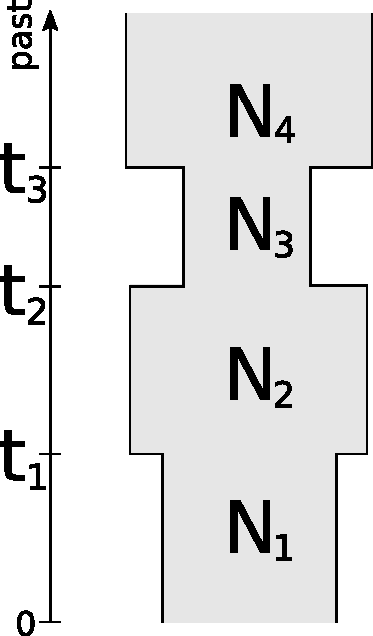
\includegraphics[width=0.25\textwidth]{graphics/piecewiseConst.pdf}
  \end{center} 
  \caption{A piecewise constant population size history for a single population. The sizes are given by $N_1$, $N_2$, $N_3$, and $N_4$. The change-times are $t_1$, $t_2$, and $t_3$.}
  \label{fig_piecewise_const}
\end{wrapfigure}

The times for the boundaries of the epochs, the populations sizes, the migration rates, the instantaneous migration probabilities and the exponential growth rates can be provided in the demography-file as outlined in the previous section. If specific values are provided in the demography-file (and rates-file), then these values are used for the entire analysis and do not change. To indicate that a certain parameter should be estimate instead of fixed for the entire analysis, you need to provide a question mark followed by a number instead of the specific value in the demography-file (or rates-file), for example, \texttt{?0}, \texttt{?1}, \texttt{?2}, and so on. The first number used in a demography-file (and rates-file) should be zero, and all numbers used should be consecutive. The number of the different parameters determine their order, which is important for specifying the initial values, for specifying boundaries, and for the output. If the same number is used twice in two different places, then these two parameters are treated as one in the optimization. That is, if a population should have the same size in two different epochs, then this can be achieved by using, for example, \texttt{?0} in both places in the demography-file. Or if migration between two sub-populations should be symmetric, then this can be achieved by using, for example, \texttt{?2} for the migration rate from $k$ to $l$, and for the migration rate from $l$ to $k$. Note that all values used in both demography-file and rates-file, if provided, are considered across files, and thus have to be compatible.

In the next sections we provide a number of example demography-file that can be used in common population genetic analyses, to further clarify the format of the demography-files. Of course, it is possible to combine different aspects of these examples for the specific application of interest.

\subsubsection{Single population: Piecewise constant population size history} 
\label{sec_demo_piecewise_constant}

% \begin{figure}
% 	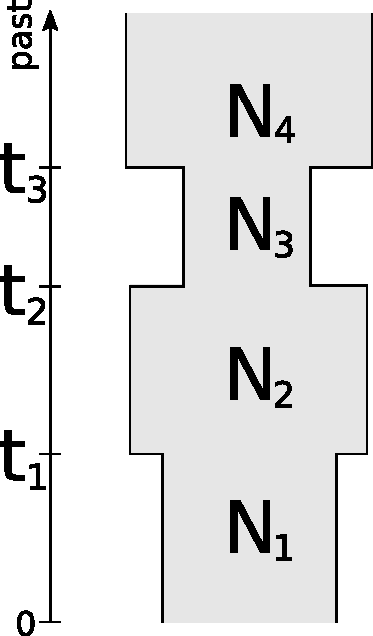
\includegraphics[width=.3\textwidth]{graphics/piecewiseConst.pdf}
% 	\caption{Something}
% 	\label{fig_isolation_migration_window}
% \end{figure}

The following demography-file describes the scenario of a single panmictic population with a piecewise constant size history, depicted in Figure~\ref{fig_piecewise_const}. In the given scenario, the size history comprises of 4 epochs, and the population size is constant in each epoch. The most recent size is $N_1$, and the size of the population changes to $N_2$ at time $t_1$ before present, and so forth. The first (non-comment) line in the file lists the three times 0.1, 0.2, and 0.4 delimiting the epochs. Recall that these are in population rescaled coalescent-time, that is, 0.1 corresponds to $0.1 \cdot 2 N_r = 2,000$ generation before present.

The line specifying the times is followed by 4 blocks, one per epoch. In each block, there is only one population that is identified with the one extant population, and thus the partition is given as \texttt{\{\{0\}\}}. The next element in each block is the constant size during this epoch, in this example given by the \texttt{?}-notation. The last two elements are the instantaneous migration probabilities, '\texttt{null}' because no instantaneous migration should happen, followed by the migration rates, given as \texttt{0}, because no continuous migration should happen. Note that in this particular demography-file, the times when the epochs change are fixed, and thus are not inferred in the analysis. The population sizes, on the other hand, are given by \texttt{?0}, \texttt{?1}, \texttt{?2}, and \texttt{?3}, indicating that these 4 parameters should be estimated.

\begin{verbatim}
PIECEWISE_CONSTANT.DEMO:

# boundary points of the epochs
#    [0,t_1,...,t_{e-1},infinity)
#    [intervals of constant demography]
[ 0.1, 0.2, 0.4 ]
# EPOCH 1
# population structure
{{0}}
# population sizes
?0
# instantaneous migration rates at beginning of epoch
null
# migration rates during epoch
0
# EPOCH 2
# population structure
{{0}}
# population sizes
?1
# instantaneous migration rates at beginning of epoch
null
# migration rates during epoch
0
# EPOCH 3
# population structure
{{0}}
# population sizes
?2
# instantaneous migration rates at beginning of epoch
null
# migration rates during epoch
0
# EPOCH 4
# population structure
{{0}}
# population sizes
?3
# instantaneous migration rates at beginning of epoch
null
# migration rates during epoch
0
\end{verbatim}

\subsubsection{Single population: Exponential growth}
\label{sec_demo_exp_growth}

% \begin{figure}
% 	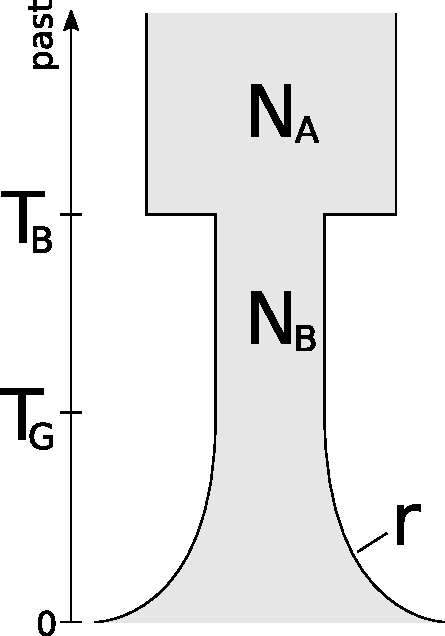
\includegraphics[width=.3\textwidth]{graphics/exp.pdf}
% 	\caption{Something}
% 	\label{fig_isolation_migration_window}
% \end{figure}

The following demography-file describes the scenario of a single panmictic population with a piecewise constant size history in the past, but a recent exponential expansion, depicted in Figure~\ref{fig_exp_growth}. In this scenario, the size history comprises of 3 epochs. The population size is constant in the two most ancient epochs, but it increases exponentially in the most recent epoch. The first (non-comment) line in the file lists the two times 0.1 and 0.4 that delimit the three epochs. Recall that these are in population rescaled coalescent-time, that is, 0.1 corresponds to $0.1 \cdot 2 N_r = 2,000$ generation before present.
% The population size before the onset of exponential growth and during the second epoch is $N_B$, whereas $N_A$ is the size of the ancestral population.

The line specifying the times is followed by 3 blocks, one per epoch. In each block, there is, again, only one population that is identified with the one extant population, and thus the partition is given as \texttt{\{\{0\}\}}. The next element in each block is the constant size during this epoch. In the first two epochs, this size is given as \texttt{?0}, indicating that this parameter should be estimated. Note that the identifier \texttt{?0} is used twice.
\begin{wrapfigure}[10]{r}{0.35\textwidth}
  \begin{center}
    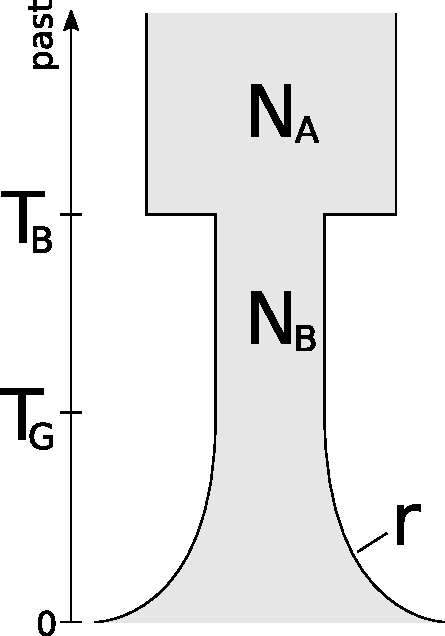
\includegraphics[width=0.25\textwidth]{graphics/exp.pdf}
  \end{center} 
  \caption{A scenario of a population size history with a bottleneck followed by recent exponential growth. The ancient population size is $N_A$, which drops to $N_B$ during the bottleneck. However, more recently it expanded at an exponential rate of $r$ The time of onset of the bottleneck is $T_B$, and the time that the exponential growth starts is denoted by $T_G$.}
  \label{fig_exp_growth}
\end{wrapfigure}
Thus, there is only a single parameter to be estimated here that determines the size in both epochs. Note further, that the size in the most recent epoch is the size at the onset of the exponential growth, and the size increases at the given rate towards the present. The ancestral size is just given as 1, and thus set equal to the reference size $N_r$. Again, the last two elements in each block are the instantaneous migration probabilities, '\texttt{null}' because no instantaneous migration should happen, followed by the migration rates, given as \texttt{0}, because there is no continuous migration.

\begin{verbatim}
EXP_GROWTH.DEMO:

# boundary points of the epochs
#    [0,t_1,...,t_{e-1},infinity)
#    [intervals of constant demography]
[ 0.1, 0.4 ]
# EPOCH 1
# population structure
{{0}}
# population sizes
?0
# instantaneous migration rates at beginning of epoch
null
# migration rates during epoch
0
# EPOCH 2
# population structure
{{0}}
# population sizes
?0
# instantaneous migration rates at beginning of epoch
null
# migration rates during epoch
0
# EPOCH 3
# population structure
{{0}}
# population sizes
1
# instantaneous migration rates at beginning of epoch
null
# migration rates during epoch
0
\end{verbatim}

To model exponential growth in this scenario, a rates-file needs to be specified in addition to the demography-file. In this case the rates-file has 3 lines, one for each epoch, and one value on each line, since in each epoch there is only one population. The growth rates in the two more ancient epochs is set to 0, since no exponential growth should happen in these epochs. The exponential growth rate in the most recent epoch is given as \texttt{?1}, indicating that this parameter should be estimated. Overall, these two files specify an exponential growth scenario with two parameters to be estimated, the population size during the bottleneck \texttt{?0} (and the size at the onset of growth), and the growth rate \texttt{?1}.

\begin{verbatim}
EXP_GROWTH.RATES:

# GROWTH RATE EPOCH 1
?1
# GROWTH RATE EPOCH 2
0
# GROWTH RATE EPOCH 3
0
\end{verbatim}

\subsubsection{Two populations: Clean split}
\label{sec_demo_clean_split}

% \begin{figure}
% 	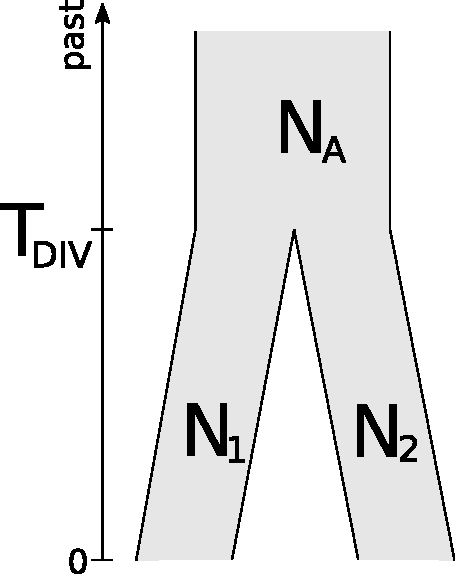
\includegraphics[width=.3\textwidth]{graphics/cleanSplit.pdf}
% 	\caption{Something}
% 	\label{fig_clean_split}
% \end{figure}

The following demography-file describes the scenario of an ancestral population that splits into two extant population at a given time before the present, depicted in Figure~\ref{fig_clean_split}. In this scenario, there are two epochs, the sizes of all populations are constant in all epochs.
% The size of the ancestral population is $N_A$, and the sizes of the two extant populations $N_1$ and $N_2$.

\begin{wrapfigure}[20]{r}{0.35\textwidth}
  \begin{center}
    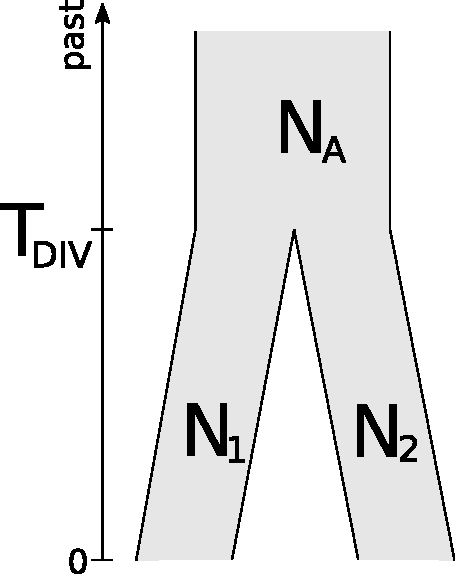
\includegraphics[width=0.25\textwidth]{graphics/cleanSplit.pdf}
  \end{center} 
  \caption{A demographic scenario where an ancestral population of size $N_A$ splits into two extant populations of size $N_1$ and $N_2$ at time $T_\text{DIV}$ before present.}
  \label{fig_clean_split}
\end{wrapfigure}

The corresponding demography-file has a list of times on the first line. Since there are only two epochs, only one time needs to be specified, which is the time of the population split. Note that here this time is given as \texttt{?0}, indicating that this time should be estimated. The line where the time is specified is followed by two blocks for each of the two epochs. The partition in the block for the more recent epoch is \texttt{\{\{0\},\{1\}\}}, indicating that there are two extant populations. The next line gives their sizes as \texttt{?1 ?2}, thus the sizes will be estimated as the second and third parameter. There is no migration between these two extant populations, so the instantaneous migration matrix is given as '\texttt{null},' and the migration rates are given as a $2 \times 2$ square matrix of zeros.

The partition in the more ancient epoch is given as \texttt{\{\{0,1\}\}}. This specifies, that the one population present in this epoch is ancestral to the two extant populations from the more recent epoch. The size of this ancestral population is given as \texttt{?3}, thus it is also estimated. Again, the migration matrices are '\texttt{null}' and 0, since no migration happens.

\begin{verbatim}
# boundary points of the epochs
#    [0,t_1,...,t_{e-1},infinity)
#    [intervals of constant demography]
[ ?0 ]
# EPOCH 1a
# population structure
{{0},{1}}
# population sizes
?1	?2
# instantaneous migration rates at beginning of epoch
null
# migration rates during epoch
0	0
0	0
# EPOCH 2
# population structure
{{0,1}}
# population sizes
?3
# instantaneous migration rates at beginning of epoch
null
# migration rates during epoch
0
\end{verbatim}

\subsubsection{Two populations: Isolation with migration}
\label{sec_demo_isolation_migration}

% \begin{figure}
% 	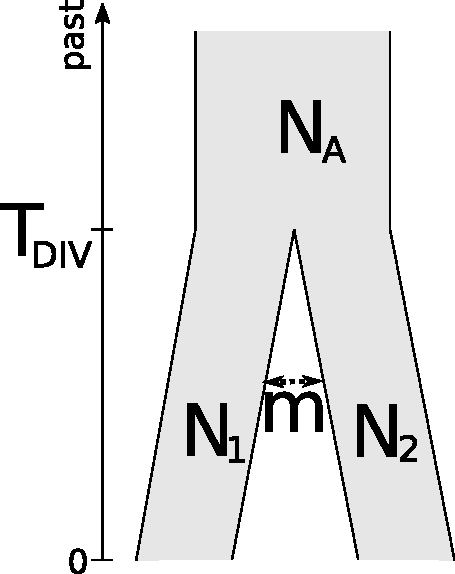
\includegraphics[width=.3\textwidth]{graphics/isolationMigration.pdf}
% 	\caption{Something}
% 	\label{fig_isolation_migration}
% \end{figure}

The following demography-file describes an isolation-with-migration (IM) scenario, that is, a scenario where an ancestral population splits into two extant population at a given time before the present, with subsequent gene-flow until the present. The scenario is depicted in Figure~\ref{fig_isolation_migration}. In this scenario, there are two epochs, the sizes of all populations are constant in all epochs.
% The size of the ancestral population is $N_A$, and the sizes of the two extant populations $N_1$ and $N_2$. The migration rate for the gene-flow that continues up to the present is denoted by $m$.

\begin{wrapfigure}[25]{r}{0.35\textwidth}
  \begin{center}
    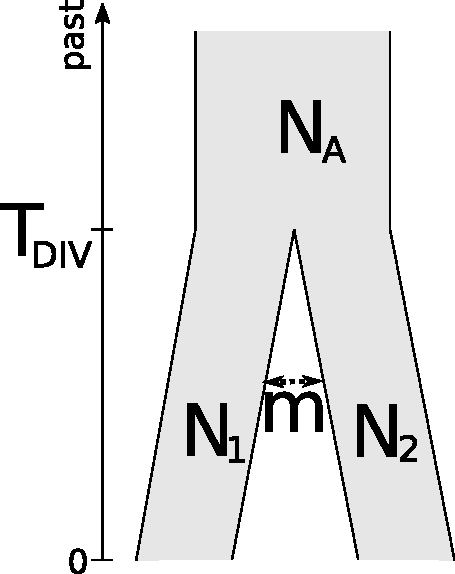
\includegraphics[width=0.25\textwidth]{graphics/isolationMigration.pdf}
  \end{center} 
  \caption{An isolation-with-migration (IM) scenario where an ancestral population of size $N_A$ splits into two extant populations of size $N_1$ and $N_2$ at time $T_\text{DIV}$ before present, with subsequent continuous gene-flow of magnitude $m$ until the present.}
  \label{fig_isolation_migration}
\end{wrapfigure}

The corresponding demography-file has a list of times on the first line. Since there are only two epochs, only one time needs to be specified, which is the time of the population split. Note that here this time is given as \texttt{?0}, indicating that this time should be estimated. The line where the time is specified is followed by two blocks for each of the two epochs. The partition in the block for the more recent epoch is \texttt{\{\{0\},\{1\}\}}, indicating that there are two extant populations. The next line gives their sizes as \texttt{?1 ?2}, thus the sizes will be estimated as the second and third parameter. There is no instantaneous migration between these two extant populations, so the instantaneous migration matrix is given as '\texttt{null}.' However, continuous gene-flow between the two extant populations is possible. Thus, the migration matrix is given by a $2 \times 2$ square matrix, with 0 on the diagonal, and \texttt{?3} for the two off-diagonal elements. Using the \texttt{?}-notation indicates that the migration rate should be estimated. Furthermore, the fact that \texttt{?3} is used for the migration rate from the first population to the second, but also for the reverse, specifies that a single parameter should be estimated for these two rates, and thus, migration is symmetric.

The partition in the more ancient epoch is given as \texttt{\{\{0,1\}\}}. This specifies, that the one population present in this epoch is ancestral to the two extant populations from the more recent epoch. The size of this ancestral population is given as \texttt{?4}, thus it is also estimated. The migration matrices are '\texttt{null}' and 0, since no migration happens in the more ancient epoch.

\begin{verbatim}
ISOLATION_MIGRATION.DEMO:

# boundary points of the epochs
#    [0,t_1,...,t_{e-1},infinity)
#    [intervals of constant demography]
[ ?0 ]
# EPOCH 1b
# population structure
{{0},{1}}
# population sizes
?1	?2
# instantaneous migration rates at beginning of epoch
null
# migration rates during epoch
0	?3
?3	0
# EPOCH 2
# population structure
{{0,1}}
# population sizes
?4
# instantaneous migration rates at beginning of epoch
null
# migration rates during epoch
0
\end{verbatim}

\subsubsection{Two populations: Isolation with migration window}
\label{sec_demo_isolation_migration_window}

% \begin{figure}
% 	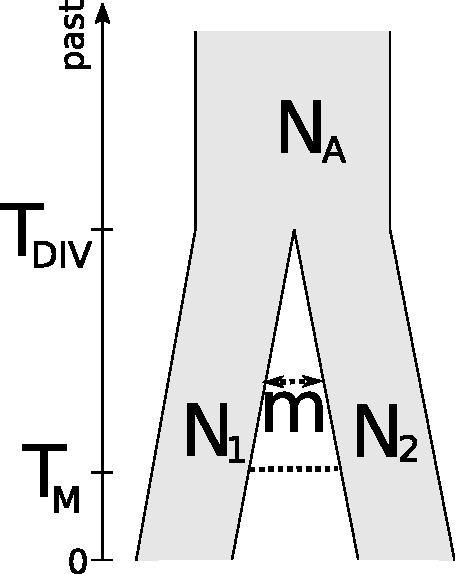
\includegraphics[width=.3\textwidth]{graphics/isolationMigrationWindow.pdf}
% 	\caption{Something}
% 	\label{fig_isolation_migration_window}
% \end{figure}

The following demography-file describes an isolation-with-migration scenario where the gene-flow stops. Specifically, in this scenario, an ancestral population splits into two extant population at a given time before the present, with subsequent gene-flow until a given time before present. The scenario is depicted in Figure~\ref{fig_isolation_migration_window}. In this scenario, there are three epochs, the sizes of all populations are constant in all epochs.
% The size of the ancestral population is $N_A$, and the sizes of the two extant populations $N_1$ and $N_2$. The migration rate for the gene-flow that stops at a given time is denoted by $m$.

\begin{wrapfigure}[24]{r}{0.35\textwidth}
  \begin{center}
    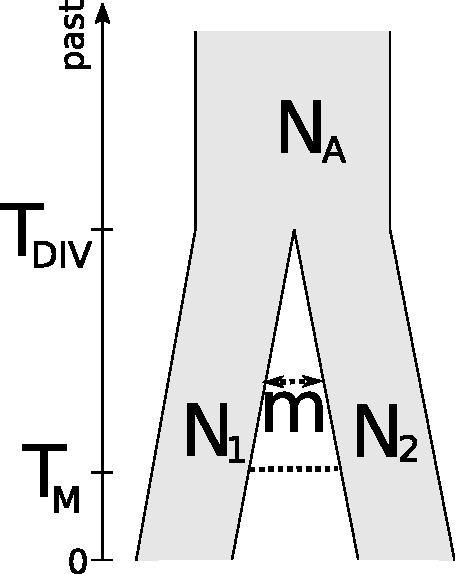
\includegraphics[width=0.25\textwidth]{graphics/isolationMigrationWindow.pdf}
  \end{center} 
  \caption{An isolation-with-migration scenario where an ancestral population of size $N_A$ splits into two extant populations of size $N_1$ and $N_2$ at time $T_\text{DIV}$ before present, with subsequent gene-flow of magnitude $m$ which lasts from $T_\text{DIV}$ until $T_\text{M}$ and then stops.}
  \label{fig_isolation_migration_window}
\end{wrapfigure}

The corresponding demography-file has a list of times on the first line. There are three epochs, and thus, two times need to be specified:  the time that the gene-flow stops and the time that the ancestral population splits. These times are given as \texttt{?0} and \texttt{?1}, indicating that these times should be estimated. The line where the times are specified is followed by three blocks for each of the three epochs. The partition in the block for the most recent epoch is \texttt{\{\{0\},\{1\}\}}, indicating that there are two extant populations. The next line gives the sizes as \texttt{?2 ?3}, thus the sizes will be estimated. There is no migration between these two extant populations in the most recent epoch, so the instantaneous migration matrix is given as '\texttt{null},' and the migration rates are given as a $2 \times 2$ square matrix of all zeros.

In the epoch in the middle, the partition is given as \texttt{\{\{0\},\{1\}\}}. Thus, in this epoch, there are again two populations, and each of them is identified with one of the two populations from the most recent epoch. Furthermore, the population sizes are given as \texttt{?2 ?3}, and thus the sizes of these populations are identical to their respective sizes in the most recent epoch, and are estimated as one parameter each. There is no instantaneous migration between these two populations in the middle epoch, so the instantaneous migration matrix is given as '\texttt{null}.' However, continuous gene-flow between these two populations is possible in the middle epoch. Thus, the migration matrix is given by a $2 \times 2$ square matrix, with 0 on the diagonal, and \texttt{?4} for the two off-diagonal elements. Using the \texttt{?}-notation indicates that the migration rate should be estimated. Furthermore, the fact that \texttt{?4} is used for the migration rate from the first population to the second, but also for the reverse, specifies that a single parameter should be estimated for these two rates, and thus, migration is symmetric.

The partition in the most ancient epoch is given as \texttt{\{\{0,1\}\}}. This specifies, that the one population present in this epoch is ancestral to the two extant populations. The size of this ancestral population is given as \texttt{?5}, thus it is also estimated. The migration matrices are '\texttt{null}' and 0, since no migration happens in the most ancient epoch.

\begin{verbatim}
ISOLATION_MIGRATION_WINDOW.DEMO:

# boundary points of the epochs
#    [0,t_1,...,t_{e-1},infinity)
#    [intervals of constant demography]
[ ?0, ?1 ]
# EPOCH 1a
# population structure
{{0},{1}}
# population sizes
?2	?3
# instantaneous migration rates at beginning of epoch
null
# migration rates during epoch
0	0
0	0
# EPOCH 1b
# population structure
{{0},{1}}
# population sizes
?2	?3
# instantaneous migration rates at beginning of epoch
null
# migration rates during epoch
0	?4
?4	0
# EPOCH 2
# population structure
{{0,1}}
# population sizes
?5
# instantaneous migration rates at beginning of epoch
null
# migration rates during epoch
0
\end{verbatim}

\subsubsection{Three populations: Divergence times}
\label{sec_demo_three_populations}

% \begin{figure}
% 	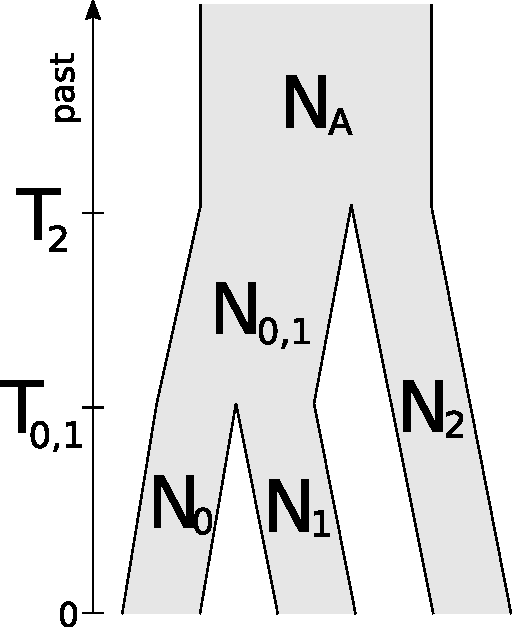
\includegraphics[width=.3\textwidth]{graphics/threePop.pdf}
% 	\caption{Something}
% 	\label{fig_three_pop}
% \end{figure}

The following demography-file describes a scenario with three extant populations, depicted in Figure~\ref{fig_three_pop}. In this scenario, and ancestral population of size $N_A$ splits into two populations at time $T_2$ before present, one of size $N_{0,1}$ and one of size $N_2$. Subsequently, at time $T_{0,1}$ before present, the population of size $N_{0,1}$ splits again into two populations of sizes $N_0$ and $N_1$, resulting in three extant populations at present. The corresponding demography-file has a list of times on the first line. There are three epochs, and thus, two times need to be specified: the time that the intermediate population splits into the two extant populations, and the time that the ancestral population splits into two. These times are given as \texttt{?0} and \texttt{?1}, indicating that these times should be estimated.

The line where the times are specified is followed by three blocks for each of the three epochs. The partition in the block for the most recent epoch is \texttt{\{\{0\},\{1\},\{2\}\}}, indicating that there are three extant populations. The next line gives the sizes for the three populations as three ones. Thus, the sizes of the extant populations are given by the reference size $N_r$. There is no migration between these three extant populations in the most recent epoch, so the instantaneous migration matrix is given as '\texttt{null},' and the migration rates are given as a $3 \times 3$ square matrix of all zeros.

\begin{wrapfigure}[15]{r}{0.35\textwidth}
  \begin{center}
    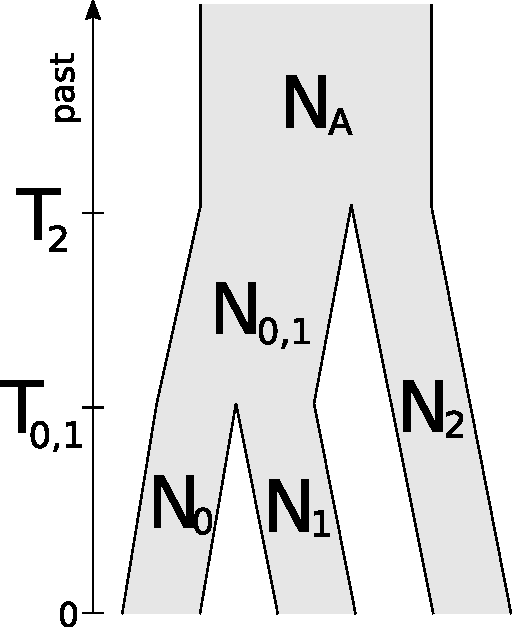
\includegraphics[width=0.25\textwidth]{graphics/threePop.pdf}
  \end{center} 
  \caption{A demographic scenario where an ancestral population of size $N_A$ splits into two populations of sizes $N_{0,1}$ and $N_2$ at time $T_2$ before present. The population $N_{0,1}$ furthermore splits into two populations of sizes $N_0$ and $N_1$ at time $T_{0,1}$.}
  \label{fig_three_pop}
\end{wrapfigure}

In the epoch in the middle, the partition is given as \texttt{\{\{0,1\},\{2\}\}}. Thus, in this epoch, there are two populations. The first population is ancestral to the first two populations from the most recent epoch, and the last population is identified with the last population from the most recent epoch. The next line gives the sizes for the two populations as two ones. Thus, the sizes of the two populations are again given by the reference size $N_r$. There is no migration between the two populations, so the instantaneous migration matrix is given as '\texttt{null},' and the migration rates are given as a $2 \times 2$ square matrix of all zeros.

The partition in the most ancient epoch is given as \texttt{\{\{0,1,2\}\}}. This specifies, that the one population present in this epoch is ancestral to the two populations from the middle epoch. The size of this ancestral population is given as 1, thus equal to the reference size $N_r$. The migration matrices are '\texttt{null}' and 0, since no migration happens in the most ancient epoch.

\begin{verbatim}
THREE_POPULATIONS.DEMO:

# boundary points of the epochs
#    [0,t_1,...,t_{e-1},infinity)
#    [intervals of constant demography]
[ ?0, ?1 ]
# EPOCH 1
# population structure
{{0},{1},{2}}
# population sizes
1 1 1
# instantaneous migration rates at beginning of epoch
null
# migration rates during epoch
0	0	0
0	0	0
0	0	0
# EPOCH 2
# population structure
{{0,1},{2}}
# population sizes
1 1
# instantaneous migration rates at beginning of epoch
null
# migration rates during epoch
0	0
0	0
# EPOCH 3
# population structure
{{0,1,2}}
# population sizes
1
# instantaneous migration rates at beginning of epoch
null
# migration rates during epoch
0
\end{verbatim}

\subsubsection{Three populations: Introgression}
\label{sec_demo_introgression}

% \begin{figure}
% 	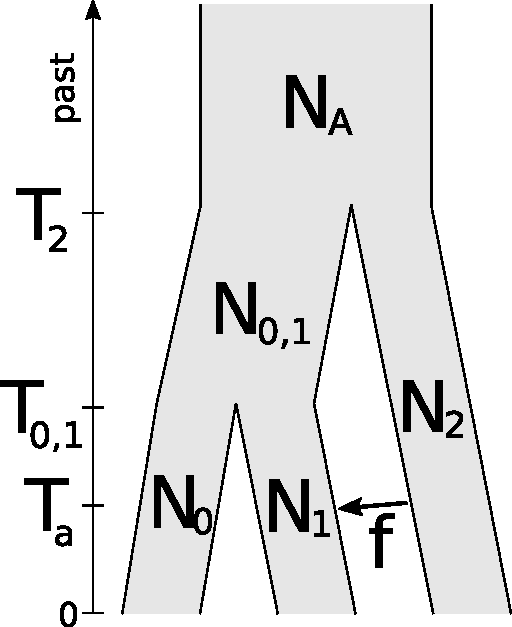
\includegraphics[width=.3\textwidth]{graphics/introgression.pdf}
% 	\caption{Something}
% 	\label{fig_introgression}
% \end{figure}

The following demography-file describes a scenario with three extant populations with introgression, depicted in Figure~\ref{fig_introgression}. In this scenario, and ancestral population of size $N_A$ splits into two populations at time $T_2$ before present, one of size $N_{0,1}$ and one of size $N_2$. Subsequently, at time $T_{0,1}$ before present, the population of size $N_{0,1}$ splits again into two populations of sizes $N_0$ and $N_1$, resulting in three extant populations at present. Lastly, at time $T_a$ before present, individuals from population $N_2$ introgress into population $N_1$.

\begin{wrapfigure}[26]{r}{0.35\textwidth}
  \begin{center}
    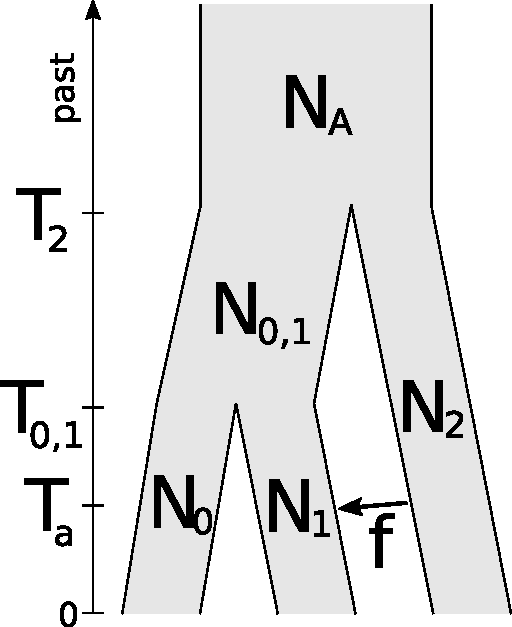
\includegraphics[width=0.25\textwidth]{graphics/introgression.pdf}
  \end{center} 
  \caption{A demographic scenario where an ancestral population of size $N_A$ splits into two populations of sizes $N_{0,1}$ and $N_2$ at time $T_2$ before present. The population $N_{0,1}$ furthermore splits into two populations of sizes $N_0$ and $N_1$ at time $T_{0,1}$. Additionally, population $N_2$ introgresses into $N_1$ at time $T_a$.}
  \label{fig_introgression}
\end{wrapfigure}

The corresponding demography-file has a list of times on the first line. There are four epochs, and thus, three times need to be specified: the time of introgression, the time that the intermediate population splits into the two extant populations, and the time that the ancestral population splits into two. These times are given as \texttt{?0}, 0.2, and 0.5, indicating that the time of introgression should be estimated, whereas the intermediate split time is given as 0.2, and the split of the ancestral population at time 0.5 before present. Recall that these times are in coalescent-units, thus 0.2 corresponds to $0.2 \cdot 2 N_r = 4000$ generations before present.

The line where the times are specified is followed by four blocks for each of the four epochs. The partition in the block for the most recent epoch is \texttt{\{\{0\},\{1\},\{2\}\}}, indicating that there are three extant populations. The next line gives the sizes for the three populations as three ones. Thus, the sizes of the extant populations are given by the reference size $N_r$. There is no migration between these three extant populations in the most recent epoch, so the instantaneous migration matrix is given as '\texttt{null},' and the migration rates are given as a $3 \times 3$ square matrix of all zeros.

In the next epoch, there are again three populations, each is identified with one extant population, and thus the partition is given as \texttt{\{\{0\},\{1\},\{2\}\}}. The next line gives the sizes for the three populations as three ones. Thus, again, the sizes of the three populations are equal to the reference size $N_r$. Importantly, intogression happens at the more recent time in this epoch. Thus, there is a $3 \time 3$ instantaneous migration specified for this epoch. This matrix is composed of all zeros, except for the entry at the third position in the second row. This entry gives the instantaneous migration rate from the second population to the third population, that is the probability that an individual in the second population has a parent from the third at this time, modeling introgression from the third population into the second. This entry is given as \texttt{?1}, indicating that this introgression probability should be estimated. There is no continuous migration in this epoch, thus the migration rates are given as a $3 \times 3$ square matrix of all zeros.

In the third epoch, the partition is given as \texttt{\{\{0,1\},\{2\}\}}. Thus, in this epoch, there are two populations. The first population is ancestral to the first two populations from the more recent epoch, and the last population is identified with the last population from the more recent epoch. The next line gives the sizes for the two populations as two ones. Thus, the sizes of the extant populations are again given by the reference size $N_r$. There is no migration between the two populations, so the instantaneous migration matrix is given as '\texttt{null},' and the migration rates are given as a $2 \times 2$ square matrix of all zeros.

The partition in the most ancient epoch is given as \texttt{\{\{0,1,2\}\}}. This specifies, that the one population present in this epoch is ancestral to the two populations from the more recent epoch. The size of this ancestral population is given as 1, thus equal to the reference size $N_r$. The migration matrices are '\texttt{null}' and 0, since no migration happens in the most ancient epoch.

\begin{verbatim}
INTROGRESSION.DEMO:

# boundary points of the epochs
#    [0,t_1,...,t_{e-1},infinity)
#    [intervals of constant demography]
[ ?0, 0.2, 0.5 ]
# EPOCH 1
# population structure
{{0},{1},{2}}
# population sizes
1 1 1
# instantaneous migration rates at beginning of epoch
null
# migration rates during epoch
0	0	0
0	0	0
0	0	0
# EPOCH 2
# population structure
{{0},{1},{2}}
# population sizes
1 1 1
# instantaneous migration rates at beginning of epoch
0	0	0
0	0	?1
0	0	0
# migration rates during epoch
0	0	0
0	0	0
0	0	0
# EPOCH 3
# population structure
{{0,1},{2}}
# population sizes
1 1
# instantaneous migration rates at beginning of epoch
null
# migration rates during epoch
0	0
0	0
# EPOCH 4
# population structure
{{0,1,2}}
# population sizes
1
# instantaneous migration rates at beginning of epoch
null
# migration rates during epoch
0
\end{verbatim}

\section{Output}
\label{sec_output}

The regular output of \texttt{diCal 2} is written to the console (output to \texttt{stdout}, errors to \texttt{stderr}), so if you want to save it in a file, you have to pipe it into an output-file (using for example '\texttt{\Q{ \> \<out_file\>}}' on unix). The program outputs details about how the input is processed and details of the actual analysis. Most of this output is prefaced with the '\texttt{\#}'-character, so they can be conveniently ignored, for example by appending '\texttt{| grep -v '\#'}' to the commandline on unix.

Besides the more detailed output, \texttt{diCal 2} prints one line per EM-step that is not prefaced with the '\texttt{\#}'-character. This line contains information about the results of the current EM-step. The first value is the log-likelihood achieved by the current parameters. The second value is the time (in milliseconds) that the current EM-step required. The next values on this line are the current estimates for the parameters. Recall that the \texttt{?}-notation used in the demography-file (and the rates-file) determines, how many parameters are estimated, and what exactly the respective parameter corresponds to. If, for example, \texttt{?0} is used for time between epochs, and \texttt{?1} and \texttt{?2} are used for population sizes, then there are three numbers on the line in the ouput file for the current parameter estimates. The first number is the current estimate for the time, and the next two numbers are the current estimates for the respective population sizes (all in coalscent-scale).

The last entry on the line is an id-string of the form \texttt{GENER\_STEP\_PARTICLE}. If \texttt{diCal 2} is only performing a single EM run, then \texttt{GENER} and \texttt{PARTICLE} are always 0, and only \texttt{STEP} increases with each EM-step. However, if \texttt{diCal 2} is using the genetic algorithm detailed in Section~\ref{sec_parameter_genetic_algorithm}, then \texttt{GENER} indicates the generation of the current particle, starting at zero, \texttt{STEP} gives the current EM-step that this particle is at, and \texttt{PARTICLE} indicates the id for this particle, starting at zero.

Note that in the single EM case, the output of the EM result lines is ordered, and thus the last result gives the maximum likelihood estimate (MLE). However, when running the genetic algorithm, potentially in parallel, the EM for the different particles is performed in order of their ids, so the last result printed is not necessarily the MLE. Thus, to get the MLE in the latter case, the output has to be post-processed to identify the line with the highest log-likelihood.


\section{Complete list of command line parameters}
\label{sec_command_line}

Here we describe the command line parameters for \texttt{diCal 2} in detail. In Section~\ref{sec_parameter_mandatory}, we describe the parameters that are required for each analysis. Furthermore, \texttt{diCal 2} has two different modes of operation: Single Expectation-Maximization (EM) analysis, or a genetic algorithm, that starts several instances of the EM and optimizes the parameters in parallel. The parameters for the former are described in Section~\ref{sec_parameter_em}, and the parameters for the latter are described in Section~\ref{sec_parameter_genetic_algorithm}. Lastly, optional parameters to fine-tune the analysis are described in Section~\ref{sec_parameter_optional}.

Note that some command line parameters require a list of arguments separated by ',' or ';'. In some cases, shells can interpret these delimiters as separating input, which would prohibit \texttt{diCal 2} from operating correctly. To circumvent this problem, the list of arguments need to be put into single quotation marks. That is, instead of \texttt{arg1,arg2,arg3}, you need to write \texttt{'arg1,arg2,arg3'}.

\subsection{Mandatory parameters}
\label{sec_parameter_mandatory}

Here we list the parameters that are mandatory for analyzing data using \texttt{diCal 2}. Note that some of these parameters are not strictly mandatory, but we list them here as they are strongly recommended. Note that the parameters \Q{--intervalType} and \Q{--lociPerHmmStep} determine the number of hidden states and the effective sequence length of the HMM in the analysis, respectively. Thus, few intervals or a large number of loci to group can results in a fast analysis with low accuracy, whereas a lot of intervals and a low number of loci to group increases accuracy, but can severely increase the runtime as well. We recommend starting with a number of intervals around 10 and 1000 loci to group, and then increasing or decreasing these values as needed.

The mandatory parameters are:
\begin{description}
	\item[\Q{--bounds <bounds>}] A string of semicolon separated list of pairs of doubles, each pair separated by a comma. This list gives the bounds for each parameter during the EM-estimation. The first value in each pair is the lower bound, the second the upper bound. The number of pairs has to be equal to the number of parameters to estimate. Note that these bounds have to be in coalescent-scale.
	\item[\Q{--compositeLikelihood <compositeLikelihood>}] The composite likelihood type to use for the analysis. We recommend using \texttt{LOL} (leave-one-out), \texttt{PCL} (pairwise-composite-likelihood), or \texttt{PAC} (product-of-approximate-conditionals). See Section~3 in the supplemental material from~\cite{Steinruecken2019} for more details.
	\item[\Q{(-c|--configFile) <configFile>}] The input configuration file. This file details meta parameters and which haplotypes are sampled in which sub-population. Section~\ref{sec_config} describes in detail how this file has to be composed.
	\item[\Q{--demoFile <demoFile>}] The demography parameter file that encodes the demographic model used in the analysis. Section~\ref{sec_demo} details how to compose this file.
	\item[\Q{--intervalType <intervalType>}] Specifies the time intervals used for the hidden states of the HMM. The number of hidden states increases linearly with the number of intervals. We recommend using \texttt{simple} or \texttt{loguniform}. In the former case, the time intervals are equivalent to the epochs specified in the demography-file. In the latter case, they need to be specified using the additional command line argument \Q{--intervalParams <intervalParams>} (see Section~\ref{sec_parameter_optional}). Note that this parameter determines the number of hidden states of the HMM, and thus has a severe impact on runtime and accuracy.
	\item[\Q{--lociPerHmmStep <lociPerHmmStep>}] This argument specifies the number of loci that are grouped together into blocks for the analysis. No recombination happens within a block, and recombination happens at an elevated rate between blocks. See Section~4 in the supplemental material from~\cite{Steinruecken2019} for more details. Note that this parameter determines the effective sequence length of the HMM, and thus has a severe impact on runtime and accuracy.
	\item[\Q{--numberIterationsEM <numberIterationsEM>}] The number of EM steps to be taken.
	\item[\Q{--numberIterationsMstep <numberIterationsMstep>}] The number of M-steps to be taken. Important: this number of steps is taken into each coordinate direction during parameter estimation.
	\item[\Q{(-p|--paramFile) <paramFile>}] The input parameter file. Section~\ref{sec_param} details how to format this file.
	\item[\Q{--seed <seed>}] The seed to initialize the randomness.
	\item[\Q{--vcfFile <vcfFile>}] The file providing the genomic sequences to be analyzed in VCF-format. Section~\ref{sec_vcf} details how to format this file. 
	\item[\Q{--vcfFilterPassString <vcfFilterPassString>}] The string in the FILTER column of a VCF-file that marks a SNP as having passed the filters. All other sites will be ignored during the analysis.
\end{description}

\subsection{Single EM analysis}
\label{sec_parameter_em}

One of the two modes that \texttt{diCal 2} can perform to analyze data is just a single run of the EM algorithm. The parameters in Section~\ref{sec_parameter_mandatory} regarding the number of steps apply to this single run. The E-step is computed using standard algorithms for HMMs. The M-step cannot be optimized analytically, and is thus optimized numerically using the Nelder-Mead algorithm. By default, the optimization is performed into every coordinate direction independently for the given number of steps during one iteration of the M-step. The only additional argument that need to be supplied is the starting point in the parameter space for the EM:

\begin{description}
	\item[\Q{--startPoint <startPoint>}] The starting point for the EM. The values have to be supplied as a comma-separated list. The number of values has to be equal to the number of parameters to be estimated. Note that these values have to be in coalescent-scale.
\end{description}

\subsection{Genetic algorithm}
\label{sec_parameter_genetic_algorithm}

In addition to just a single run of the EM algorithm, \texttt{diCal 2} can be applied using a simple genetic algorithm. In this algorithm, a number of particles start at given points in the parameter space. Each particle performs a number of EM-steps for optimization (specified using the respective parameters). After each particle performed their steps, the particles that achieved the highest likelihoods are chosen as the 'parents' for the next 'generation' of particles. The particles with the lower likelihoods are discarded and replaced by randomly distorted versions of the 'parents'. Several generations are repeated for a given number of times. This genetic algorithm allows a faster exploration of the parameter space and is less prone to get stuck in local optima. The different particles can be evolved in parallel, but it does increase the overall runtime. 

The parameters for the genetic algorithm are:
\begin{description}
 	\item[\Q{--metaKeepBest <metaKeepBest>}] The number of particles with the highest likelihood in a generation retained to be the 'parents' of the next generation.
 	\item[\Q{--metaNumIterations <metaNumIterations>}] The number of generations that this genetic algorithm should be repeated for.
 	\item[\Q{--metaNumPoints <metaNumPoints>}] The number of particles in each generation.
	\item[\Q{--metaParallelEmSteps <metaParallelEmSteps>}] Number of EM particles to be executed in parallel during genetic algorithm. This should only be used in conjunction with the \Q{--parallel} argument, and the number should be less than a fourth of the number of cores used to avoid reduction in performance.
	\item[\Q{--metaStartFile <metaStartFile>}] A file containing the starting points (first generation of particles). Each line in this file is for one particle. The values on each line have to be separated by whitespaces and equal to the number of parameters to be estimated (and given in coalescent-scale).
\end{description}

\subsection{Optional parameters}
\label{sec_parameter_optional}

The following optional parameters can be used to have additional control over certain aspects of the analysis, and in some cases can replace the parameters from the previous sections.

\begin{description}
	\item[\Q{--help}] Prints the usage for the software.
	\item[\Q{--bedFile <bedFile>}] *.bed file(s) that lists all regions of the VCF-file that should be EXCLUDED from the analysis.
	\item[\Q{--coordinateOrder <coordinateOrder>}] Order in which to update the parameters independently in each direction during the M-step. If not specified, use random order.
	\item[\Q{--diffPermsPerChunk}] If this switch is set, a use different set of permutations for each independent chunk.
	\item[\Q{--disableCoordinateWiseMStep}] Default mode is to update the parameters independently in each coordinate direction during the M-step. The number of iterations provided are applied coordinate-wise. This default mode is disabled by providing this flag. If disabled, the M-step optimization uses a general multidimensional NM algorithm.
	\item[\Q{--hidden}] Show all command line parameter (including hidden ones). WARNING: Experts only.
	\item[\Q{--intervalParams <intervalParams>}] The parameters for generating the time intervals for the hidden states of the HMM. Should be used in conjunction with \Q{--intervalType loguniform}. In this case, you should provide 3 comma-separated values. The first is the number of times separating the intervals. The second and third is the minimum and maximum time, respectively. The times are chosen equidistantly in log-scale between this minimum and maximum. The first interval starts at 0, and the last interval ends at infinity.
 	\item[\Q{--metaGridStart}] For genetic algorithm only: If flag is set, start with of a grid of points chosen equidistant between the bounds provided. Otherwise the start points are chosen randomly.
	\item[\Q{--metaNumStartPoints <metaNumStartPoints>}] For genetic algorithm only: The number of starting points (in each dimension if a grid is specified).
	\item[\Q{--numCsdsPerPerm <numCsdsPerPerm>}] Number of CSDs used for each permutation.
	\item[\Q{(-n|--numPerDeme) <numPerDeme>}] The number of individuals per sub-population. e.g. 5,3,2 means the first 5 haplotypes in the VCF-file are in sub-population 0, the next 3 are in sub-population 1, and the next 2 are in sub-population 2.
	\item[\Q{--numPermutations <numPermutations>}] Number of permutations to use for PAC-like methods.
	\item[\Q{--parallel <parallel>}] If supplied, the analysis is done on \Q{\<parallel\>} cpu-cores in parallel.
	\item[\Q{--permutationsFile <permutationsFile>}] Specify file(s) containing a list of permutations to be used to analyze each VCF-file respectively. Only for PAC-like methods.
	\item[\Q{--printIntervals}] If this switch is set, the time intervals used are printed.
	\item[\Q{--ratesFile <ratesFile>}] The file with the exponential growth rates. Has to match the demography file. For more details, see Section~\ref{sec_exponential}.
	\item[\Q{--vcfOffset <vcfOffset>}] Offset(s) to shift the positions given in the VCF-file(s). One value if ony one VCF-file is provided, a comma-separated list otherwise.
	\item[\Q{--vcfReferenceFile <vcfReferenceFile>}] Provide a file containing the reference sequence to be used with the VCF-file. Needs to be in fasta-format. Specifying this option overrides whatever is provided in the VCF-file. See Section~\ref{sec_reference} for more details.
	\item[\Q{-v|--verbose}] More output, especially during the EM-steps.
\end{description}   

\section{Examples}
\label{sec_examples}

In this section, we exhibit several examples that showcase scenarios in which \texttt{diCal 2} can be applied to infer demographic parameters. Although the Expectation-Maximization (EM) in Section~\ref{sec_examples_em}, the genetic algorithm in Section~\ref{sec_examples_genetic}, and the computation of likelihoods in Section~\ref{sec_examples_likelihood} are applied in certain demographic scenarios, these methods can certainly also be applied in all other demographic scenarios that are listed here or that can be specified as input to \texttt{diCal 2}.

Note that the settings used in these examples are primarily for the purpose of demonstrating how to run \texttt{diCal 2} in the respective scenarios. Some of these settings might have to be adjusted to achieve better efficiency and accuracy when analyzing genome-scale datasets. In particular, testing different composite likelihoods (\Q{--compositeLikelihood}) is advisable. Moreover, the number of loci to group (\Q{--lociPerHmmStep}) and the number of hidden states for the HMM (\Q{--intervalType} and \Q{--intervalParams}) in the examples are good starting points, but might have to be adjusted. Furthermore, increasing the number of steps in the EM algorithm (\Q{--numberIterationsEM} and \Q{--numberIterationsMstep}) can result in better estimates. In a similar vain, for the genetic algorithm, increasing the number of generations (\Q{--metaNumIterations}), the number of particles per generation (\Q{--metaNumPoints}), and the number retained (\Q{--metaKeepBest}) will result in longer runtime, but likely improve inference as well. The starting point(s), be it single points for the EM (\Q{--startPoint}) or a list of points for the genetic algorithm (\Q{--metaStartFile}), should be varied and/or increased in numbers as well. Lastly, if possible, the number of threads/cores used should be increased as well (\Q{--parallel}).

The input files for the examples can be found after extracting the archive downloaded from \url{https://sourceforge.net/projects/dical2/} in the subdirectory \texttt{examples}. The download does not include the simulated genetic data necessary to run the examples, but python-scripts to simulate the data using \texttt{msprime} are included. Thus, the simulation scripts should be run before running the examples.


\subsection{Parameter estimation - Expectation Maximization (EM)}
\label{sec_examples_em}

The following examples showcase applications of the Expectation-Maximization (EM) algorithm, where the optimization starts from a given set of parameters and updates them step-by-step using the EM algorithm for HMMs.

\subsubsection{Single population: Piecewise constant population size history} 
\label{sec_examples_piecewise_constant}

The following example infers population sizes in a model of piecewise constant population size history described in Section~\ref{sec_demo_piecewise_constant}, and the files for the analysis can be found in the directory \texttt{examples/piecewiseConstant}:

\begin{verbatim}
java -jar ../../diCal2.jar --paramFile mutRec.param --vcfFile contig.0.vcf
  --vcfFilterPassString PASS --vcfReferenceFile output.ref --lociPerHmmStep 1000
  --configFile piecewise_constant.config --demoFile piecewise_constant.demo
  --intervalType loguniform --intervalParams '8,0.01,4' --compositeLikelihood pcl
  --startPoint '1,2,0.5,1' --bounds '0.01,20;0.01,20;0.01,20;0.01,20' 
  --numberIterationsEM 10 --numberIterationsMstep 5 --seed 4711 --verbose
\end{verbatim}

The mutation/recombination parameter file supplied using the \Q{--paramFile} argument is given in Section~\ref{sec_param}. The VCF-file containing the segregating sites for the haplotypes is provided using the \Q{--vcfFile} argument, and the \Q{--vcfFilterPassString} indicates that all sites where the filter column has '\texttt{PASS}' should be considered for the analysis. The reference sequence for the VCF-file is provided using \Q{--vcfReferenceFile} (see Section~\ref{sec_vcf} for additional details). For the present analysis, windows of 1000 loci are grouped together (\Q{--lociPerHmmStep}). The \Q{--configFile} is given by

\begin{verbatim}
PIECEWISE_CONSTANT.CONFIG:

# numLoci	numAlleles	numDemes	 (numLoci is ignored for vcf)
100000000	2	1
# one line for each haplotype to how many in which deme
#    (each diploid is considered as two separate haplotypes)
1
1
1
1
0
0
0
0
0
0
\end{verbatim}

This file indicates, that out of the 10 haplotypes in the provided VCF-file, only the first four should be considered for the analysis (see Section~\ref{sec_config} for more details). The argument \Q{--demoFile} points to the file describing the demographic model (see Section~\ref{sec_demo_piecewise_constant}). The arguments \Q{--intervalType} and \Q{--intervalParams} indicate that there should be 10 (8+2) time intervals determining the states of the HMM, and the delimiting times should be equidistantly distributed on a log scale between (and including) 0.01 and 4. Note that these values are coalescent rescaled, so they have to be multiplied by $2N_r$ to get the corresponding number of generations. The argument \Q{--compositeLikelihood} indicates that the pairwise-composite-likelihood (\texttt{pcl}) should be used.

The EM algorithm starts with the initial parameters '\texttt{1,2,0.5,1}' (\Q{--startPoint}). Note that the demography-file specifies that these four parameters to be estimated are the population sizes for the four epochs. Thus these values are relative to the reference population size, and, for example, \texttt{1} corresponds to a size of $N_r$. The argument \Q{--bounds} is used to specify bounds for these four parameters that cannot be exceeded during the estimation. A pair of values is specified for each, the lower and upper bound, respectively. The EM algorithm is run for 10 steps (\Q{--numberIterationsEM}) and each M-step has 5 optimization steps (\Q{--numberIterationsMstep}) in each coordinate direction. Lastly, the seed for the pseudo-random number generator is 4711 (\Q{--seed}), and the output is \Q{--verbose} to provide more detail.

\subsubsection{Single population: Exponential growth}

The following example infers the population size during a recent bottleneck and the exponential growth rate for the subsequent expansion, described in Section~\ref{sec_demo_exp_growth}, and the files for the analysis can be found in the directory \texttt{examples/expGrowth}:

\begin{verbatim}
java -jar ../../diCal2.jar --paramFile mutRec.param --vcfFile 'contig.0.vcf,contig.1.vcf'
  --vcfFilterPassString PASS --vcfReferenceFile 'output.ref,output.ref'
  --lociPerHmmStep 1000 --configFile exp_growth.config --demoFile exp_growth.demo
  --ratesFile exp_growth.rates --intervalType loguniform --intervalParams '8,0.01,4'
  --compositeLikelihood pcl --startPoint '0.8,2' --bounds '0.01,20;0.05,50'
  --numberIterationsEM 10 --numberIterationsMstep 5 --seed 4711 --verbose
\end{verbatim}

The mutation/recombination parameter file supplied using the \Q{--paramFile} argument is given in Section~\ref{sec_param}. The two VCF-files containing the segregating sites for the haplotypes for two contigs are provided using the \Q{--vcfFile} argument, and the \Q{--vcfFilterPassString} indicates that all sites where the filter column has '\texttt{PASS}' should be considered for the analysis. The two reference sequences for the VCF-files are provided using \Q{--vcfReferenceFile} (see Section~\ref{sec_vcf} for additional details). For the present analysis, windows of 1000 loci are grouped together (\Q{--lociPerHmmStep}). The \Q{--configFile} is equal to the one in the example in Section~\ref{sec_examples_piecewise_constant}, indicating, that out of the 10 haplotypes in the provided VCF-file, only the first four should be considered for the analysis (see Section~\ref{sec_config} for more details). The arguments \Q{--demoFile} and \Q{--ratesFile} point to the files describing the demographic model (see Section~\ref{sec_demo_exp_growth}). The arguments \Q{--intervalType} and \Q{--intervalParams} indicate that there should be 10 (8+2) time intervals determining the states of the HMM, and the delimiting times should be equidistantly distributed on a log scale between (and including) 0.01 and 4. Note that these values are coalescent rescaled, so they have to be multiplied by $2N_r$ to get the corresponding number of generations. The argument \Q{--compositeLikelihood} indicates that the pairwise-composite-likelihood (\texttt{pcl}) should be used.

The EM algorithm starts with the initial parameters '\texttt{0.8,2}' (\Q{--startPoint}). The first value is the exponential growth rate (in coalescent-scaled time units) and the second is the population size during the bottleneck, again, relative to the reference population size $N_r$. The argument \Q{--bounds} is used to specify bounds for these parameters that cannot be exceeded during the estimation. A pair of values is specified for each, the lower and upper bound, respectively. The EM algorithm is run for 10 steps (\Q{--numberIterationsEM}) and each M-step has 5 optimization steps (\Q{--numberIterationsMstep}) in each coordinate direction. Lastly, the seed for the pseudo-random number generator is 4711 (\Q{--seed}), and the output is \Q{--verbose} to provide more detail.

\subsubsection{Two populations: Clean split}
\label{sec_examples_clean_split}

The following example infers the divergence time and population sizes in a model of a split of an ancestral population into two extant populations without subsequent gene-flow described in Section~\ref{sec_demo_clean_split}. The files for the analysis can be found in the directory \texttt{examples/cleanSplit}:

\begin{verbatim}
java -jar ../../diCal2.jar --paramFile mutRec.param --vcfFile contig.0.vcf
  --vcfFilterPassString PASS --vcfReferenceFile output.ref --lociPerHmmStep 1000
  --configFile clean_split.config --demoFile clean_split.demo --intervalType loguniform
  --compositeLikelihood lol --intervalParams '8,0.01,4' --startPoint '0.2,0.5,0.5,1'
  --bounds '0.02,20;0.01,20;0.01,20;0.01,20' --numberIterationsEM 10
  --numberIterationsMstep 5 --seed 4711 --verbose
\end{verbatim}

The mutation/recombination parameter file supplied using the \Q{--paramFile} argument is given in Section~\ref{sec_param}. The VCF-file containing the segregating sites for the haplotypes is provided using the \Q{--vcfFile} argument, and the \Q{--vcfFilterPassString} indicates that all sites where the filter column has '\texttt{PASS}' should be considered for the analysis. The reference sequence for the VCF-file is provided using \Q{--vcfReferenceFile} (see Section~\ref{sec_vcf} for additional details). For the present analysis, windows of 1000 loci are grouped together (\Q{--lociPerHmmStep}). The \Q{--configFile} is given by

\begin{verbatim}
CLEAN_SPLIT.CONFIG:

# numLoci	numAlleles	numDemes	 (numLoci is ignored for vcf)
100000000	2	2
# one line for each haplotype to how many in which deme
#    (each diploid is considered as two separate haplotypes)
1	0
1	0
0	0
0	0
0	1
0	1
0	0
0	0
\end{verbatim}

This file indicates, that out of the 8 haplotypes in the provided VCF-file, the first two should be sampled in the first extant population, and the next two should be omitted. Haplotype 5 and 6 should be sampled in the second extant population, and the last two again omitted (see Section~\ref{sec_config} for more details). The argument \Q{--demoFile} points to the file describing the demographic model (see Section~\ref{sec_demo_clean_split}). The arguments \Q{--intervalType} and \Q{--intervalParams} indicate that there should be 10 (8+2) time intervals determining the states of the HMM, and the delimiting times should be equidistantly distributed on a log scale between (and including) 0.01 and 4. Note that these values are coalescent rescaled, so they have to be multiplied by $2N_r$ to get the corresponding number of generations. The argument \Q{--compositeLikelihood} indicates that the leave-one-out-likelihood (\texttt{lol}) should be used.

The EM algorithm starts with the initial parameters '\texttt{0.2,0.5,0.5,1}' (\Q{--startPoint}). Note that the demography-file specifies that these four parameters to be estimated are the time of the population split followed by the three population sizes. The time is given in coalescent-scaled units, thus \texttt{0.2} corresponds to $0.2 \cdot 2 N_r = 4000$ generations before present. The population sizes are given relative to the reference population size, and, for example, \texttt{0.5} corresponds to a size of $0.5 N_r$. The argument \Q{--bounds} is used to specify bounds for these four parameters that cannot be exceeded during the estimation. A pair of values is specified for each, the lower and upper bound, respectively. The EM algorithm is run for 10 steps (\Q{--numberIterationsEM}) and each M-step has 5 optimization steps (\Q{--numberIterationsMstep}) in each coordinate direction. Lastly, the seed for the pseudo-random number generator is 4711 (\Q{--seed}), and the output is \Q{--verbose} to provide more detail.

\subsection{Parameter estimation - Genetic algorithm}
\label{sec_examples_genetic}

The following examples showcase applications of the genetic algorithm. Here, several instances/particles of the EM algorithm optimization are started from several given sets of initial parameters. Each 'particle' is updated step-by-step using the EM algorithm for HMMs. After a certain number of steps, the likelihoods are compared between all particles, and only the ones achieving the highest likelihood are kept for the next generation of the genetic algorithm. The other particles are replaced by randomly distorted versions of the particles with the highest likelihoods. A given number of such generations are evolved subsequently.

\subsubsection{Two populations: Clean split}

The following example infers the divergence time and population sizes in a model of a split of an ancestral population into two extant populations without subsequent gene-flow described in Section~\ref{sec_demo_clean_split}. The files for the analysis can be found in the directory \texttt{examples/cleanSplit}:

\begin{verbatim}
java -jar ../../diCal2.jar --paramFile mutRec.param --vcfFile contig.0.vcf
  --vcfFilterPassString PASS --vcfReferenceFile output.ref --lociPerHmmStep 1000
  --configFile clean_split.config --demoFile clean_split.demo --intervalType loguniform
  --intervalParams '8,0.01,4' --compositeLikelihood lol --metaStartFile clean_split.start
  --bounds '0.02,20;0.01,20;0.01,20;0.01,20' --numberIterationsEM 4
  --numberIterationsMstep 3 --metaNumIterations 3 --metaKeepBest 2 --metaNumPoints 5
  --seed 4711 --verbose
\end{verbatim}

The mutation/recombination parameter file supplied using the \Q{--paramFile} argument is given in Section~\ref{sec_param}. The VCF-file containing the segregating sites for the haplotypes is provided using the \Q{--vcfFile} argument, and the \Q{--vcfFilterPassString} indicates that all sites where the filter column has '\texttt{PASS}' should be considered for the analysis. The reference sequence for the VCF-file is provided using \Q{--vcfReferenceFile} (see Section~\ref{sec_vcf} for additional details). For the present analysis, windows of 1000 loci are grouped together (\Q{--lociPerHmmStep}). The \Q{--configFile} is the same as in Section~\ref{sec_examples_clean_split}, indicating, that out of the 8 haplotypes in the provided VCF-file, the first two should be sampled in the first extant population, and the next two should be omitted. Haplotype 5 and 6 should be sampled in the second extant population, and the last two again omitted (see Section~\ref{sec_config} for more details). The argument \Q{--demoFile} points to the file describing the demographic model (see Section~\ref{sec_demo_clean_split}). The arguments \Q{--intervalType} and \Q{--intervalParams} indicate that there should be 10 (8+2) time intervals determining the states of the HMM, and the delimiting times should be equidistantly distributed on a log scale between (and including) 0.01 and 4. Note that these values are coalescent rescaled, so they have to be multiplied by $2N_r$ to get the corresponding number of generations. The argument \Q{--compositeLikelihood} indicates that the leave-one-out-likelihood (\texttt{lol}) should be used.

The argument \Q{--metaStartFile} provides a file with a list of starting parameter sets for the EM (one set per line, values separated by whitespaces), which looks as follows

\begin{verbatim}
CLEAN_SPLIT.START:

0.1	0.25	0.25	1
0.2	0.25	0.25	1
0.4	0.25	0.25	1
0.1	1	1	1
0.2	1	1	1
0.4	1	1	1
\end{verbatim}

Note that the demography-file specifies that the four parameters to be estimated are the time of the population split followed by the three population sizes. The time is given in coalescent-scaled units, thus \texttt{0.2} corresponds to $0.2 \cdot 2 N_r = 4000$ generations before present. The population sizes are given relative to the reference population size, and, for example, \texttt{0.25} corresponds to a size of $0.25 N_r$. The argument \Q{--bounds} is used to specify bounds for these four parameters that cannot be exceeded during the estimation. A pair of values is specified for each, the lower and upper bound, respectively. For each initial set of parameters, the EM algorithm is run for 4 steps (\Q{--numberIterationsEM}) and each M-step has 3 optimization steps (\Q{--numberIterationsMstep}) in each coordinate direction. After this, the 2 particles with the highest likelihood are kept (\Q{--metaKeepBest}), and 2 additional generations (\Q{--metaNumIterations 3}) with 5 particles each (\Q{--metaNumPoints}) are optimized. Lastly, the seed for the pseudo-random number generator is 4711 (\Q{--seed}), and the output is \Q{--verbose} to provide more detail.

\subsubsection{Two populations: Isolation with migration}

The following example infers the divergence time, symmetric migration rate, and population sizes in a model of a split of an ancestral population into two extant populations with subsequent gene-flow described in Section~\ref{sec_demo_isolation_migration}. The files for the analysis can be found in the directory \texttt{examples/isolationMigration}:

\begin{verbatim}
java -jar ../../diCal2.jar --paramFile mutRec.param --vcfFile contig.0.vcf
  --vcfFilterPassString PASS --vcfReferenceFile output.ref --lociPerHmmStep 1000
  --configFile isolation_migration.config --demoFile isolation_migration.demo
  --intervalType loguniform --intervalParams '8,0.01,4' --compositeLikelihood lol
  --metaStartFile isolation_migration.start
  --bounds '0.02,20;0.01,20;0.01,20;0.01,100;0.01,20' --numberIterationsEM 4
  --numberIterationsMstep 3 --metaNumIterations 3 --metaKeepBest 2 --metaNumPoints 5
  --seed 4711 --verbose
\end{verbatim}

The mutation/recombination parameter file supplied using the \Q{--paramFile} argument is given in Section~\ref{sec_param}. The VCF-file containing the segregating sites for the haplotypes is provided using the \Q{--vcfFile} argument, and the \Q{--vcfFilterPassString} indicates that all sites where the filter column has '\texttt{PASS}' should be considered for the analysis. The reference sequence for the VCF-file is provided using \Q{--vcfReferenceFile} (see Section~\ref{sec_vcf} for additional details). For the present analysis, windows of 1000 loci are grouped together (\Q{--lociPerHmmStep}). The \Q{--configFile} is the same as in Section~\ref{sec_examples_clean_split}, indicating, that out of the 8 haplotypes in the provided VCF-file, the first two should be sampled in the first extant population, and the next two should be omitted. Haplotype 5 and 6 should be sampled in the second extant population, and the last two again omitted (see Section~\ref{sec_config} for more details). The argument \Q{--demoFile} points to the file describing the demographic model (see Section~\ref{sec_demo_isolation_migration}). The arguments \Q{--intervalType} and \Q{--intervalParams} indicate that there should be 10 (8+2) time intervals determining the states of the HMM, and the delimiting times should be equidistantly distributed on a log scale between (and including) 0.01 and 4. Note that these values are coalescent rescaled, so they have to be multiplied by $2N_r$ to get the corresponding number of generations. The argument \Q{--compositeLikelihood} indicates that the leave-one-out-likelihood (\texttt{lol}) should be used.

The argument \Q{--metaStartFile} provides a file with a list of starting parameter sets for the EM (one set per line, values separated by whitespaces), which looks as follows

\begin{verbatim}
ISOLATION_MIGRATION.START:

0.1	0.25	0.25	0.1	1
0.4	0.25	0.25	0.1	1
0.1	1	1	0.1	1
0.4	1	1	0.1	1
0.1	0.25	0.25	10	1
0.4	0.25	0.25	10	1
0.1	1	1	10	1
0.4	1	1	10	1
\end{verbatim}

Note that the demography-file specifies that the five parameters to be estimated are the time of the population split, followed by the two extant population sizes, the migration rate, and the size of the ancestral population. The time is given in coalescent-scaled units, thus \texttt{0.4} corresponds to $0.4 \cdot 2 N_r = 8000$ generations before present. The population sizes are given relative to the reference population size, and, for example, \texttt{0.25} corresponds to a size of $0.25 N_r$. The migration rate is also population-rescaled, thus \texttt{0.1} corresponds to a per generation probability of $\frac{0.1}{4 N_r} = 0.0000025$ that an individual's parent is a migrant. The argument \Q{--bounds} is used to specify bounds for these five parameters that cannot be exceeded during the estimation. A pair of values is specified for each, the lower and upper bound, respectively. For each initial set of parameters, the EM algorithm is run for 4 steps (\Q{--numberIterationsEM}) and each M-step has 3 optimization steps (\Q{--numberIterationsMstep}) in each coordinate direction. After this, the 2 particles with the highest likelihood are kept (\Q{--metaKeepBest}), and 2 additional generations (\Q{--metaNumIterations 3}) with 5 particles each (\Q{--metaNumPoints}) are optimized. Lastly, the seed for the pseudo-random number generator is 4711 (\Q{--seed}), and the output is \Q{--verbose} to provide more detail.

\subsubsection{Two populations: Isolation with migration window}

The following example infers the migration window, divergence time, symmetric migration rate, and population sizes in a model of a split of an ancestral population into two extant populations with subsequent gene-flow that stops described in Section~\ref{sec_demo_isolation_migration_window}. The files for the analysis can be found in the directory \texttt{examples/isolationMigrationWindow}:

\begin{verbatim}
java -jar ../../diCal2.jar --paramFile mutRec.param --vcfFile contig.0.vcf
  --vcfFilterPassString PASS --vcfReferenceFile output.ref --lociPerHmmStep 1000
  --configFile isolation_migration_window.config
  --demoFile isolation_migration_window.demo --intervalType loguniform
  --intervalParams '8,0.01,4' --compositeLikelihood lol
  --metaStartFile isolation_migration_window.start
  --bounds '0.02,20;0.02,20;0.01,20;0.01,20;0.01,100;0.01,20' --numberIterationsEM 4
  --numberIterationsMstep 3 --metaNumIterations 3 --metaKeepBest 2 --metaNumPoints 5
  --seed 4711 --verbose --metaParallelEmSteps 2 --parallel 4
\end{verbatim}

The mutation/recombination parameter file supplied using the \Q{--paramFile} argument is given in Section~\ref{sec_param}. The VCF-file containing the segregating sites for the haplotypes is provided using the \Q{--vcfFile} argument, and the \Q{--vcfFilterPassString} indicates that all sites where the filter column has '\texttt{PASS}' should be considered for the analysis. The reference sequence for the VCF-file is provided using \Q{--vcfReferenceFile} (see Section~\ref{sec_vcf} for additional details). For the present analysis, windows of 1000 loci are grouped together (\Q{--lociPerHmmStep}). The \Q{--configFile} is the same as in Section~\ref{sec_examples_clean_split}, indicating, that out of the 8 haplotypes in the provided VCF-file, the first two should be sampled in the first extant population, and the next two should be omitted. Haplotype 5 and 6 should be sampled in the second extant population, and the last two again omitted (see Section~\ref{sec_config} for more details). The argument \Q{--demoFile} points to the file describing the demographic model (see Section~\ref{sec_demo_isolation_migration_window}). The arguments \Q{--intervalType} and \Q{--intervalParams} indicate that there should be 10 (8+2) time intervals determining the states of the HMM, and the delimiting times should be equidistantly distributed on a log scale between (and including) 0.01 and 4. Note that these values are coalescent rescaled, so they have to be multiplied by $2N_r$ to get the corresponding number of generations. The argument \Q{--compositeLikelihood} indicates that the leave-one-out-likelihood (\texttt{lol}) should be used.

The argument \Q{--metaStartFile} provides a file with a list of starting parameter sets for the EM (one set per line, values separated by whitespaces), which looks as follows

\begin{verbatim}
ISOLATION_MIGRATION_WINDOW.START:

0.1	0.2	0.25	0.25	0.1	1
0.1	0.4	0.25	0.25	0.1	1
0.1	0.2	1	1	0.1	1
0.1	0.4	1	1	0.1	1
0.1	0.2	0.25	0.25	10	1
0.1	0.4	0.25	0.25	10	1
0.1	0.2	1	1	10	1
0.1	0.4	1	1	10	1
\end{verbatim}

Note that the demography-file specifies that the six parameters to be estimated are the time that the migration stops, the time of the population split, the two extant population sizes, the migration rate, and the size of the ancestral population. The times are given in coalescent-scaled units, thus \texttt{0.4} corresponds to $0.4 \cdot 2 N_r = 8000$ generations before present. The population sizes are given relative to the reference population size, and, for example, \texttt{0.25} corresponds to a size of $0.25 N_r$. The migration rate is also population-rescaled, thus \texttt{0.1} corresponds to a per generation probability of $\frac{0.1}{4 N_r} = 0.0000025$ that an individual's parent is a migrant. The argument \Q{--bounds} is used to specify bounds for these six parameters that cannot be exceeded during the estimation. A pair of values is specified for each, the lower and upper bound, respectively. For each initial set of parameters, the EM algorithm is run for 4 steps (\Q{--numberIterationsEM}) and each M-step has 3 optimization steps (\Q{--numberIterationsMstep}) in each coordinate direction. After this, the 2 particles  with the highest likelihood are kept (\Q{--metaKeepBest}), and 2 additional generations (\Q{--metaNumIterations 3}) with 5 particles each (\Q{--metaNumPoints}) are optimized. The seed for the pseudo-random number generator is 4711 (\Q{--seed}), and the output is \Q{--verbose} to provide more detail. Lastly, the program is allowed to use 4 parallel threads on different cpu-cores (\Q{--parallel}) and 2 EM particles are optimized in parallel (\Q{--metaParallelEmSteps}).

\subsubsection{Three populations: Divergence times}
\label{sec_examples_three_populations}

The following example infers the divergence times in a scenario where an ancestral population splits into two populations, one of which splits again into two at a more recent time, described in Section~\ref{sec_demo_three_populations}. The files for the analysis can be found in the directory \texttt{examples/threePopulations}:

\begin{verbatim}
java -jar ../../diCal2.jar --paramFile mutRec.param  --vcfFile contig.0.vcf
  --vcfFilterPassString PASS --vcfReferenceFile output.ref --lociPerHmmStep 1000
  --configFile three_populations.config --demoFile three_populations.demo
  --intervalType loguniform --intervalParams '8,0.01,4'  --compositeLikelihood lol
  --metaStartFile three_populations.start --bounds '0.02,20;0.02,20' --numberIterationsEM 4
  --numberIterationsMstep 3 --metaNumIterations 3 --metaKeepBest 2 --metaNumPoints 5
  --seed 4711 --verbose
\end{verbatim}

The mutation/recombination parameter file supplied using the \Q{--paramFile} argument is given in Section~\ref{sec_param}. The VCF-file containing the segregating sites for the haplotypes is provided using the \Q{--vcfFile} argument, and the \Q{--vcfFilterPassString} indicates that all sites where the filter column has '\texttt{PASS}' should be considered for the analysis. The reference sequence for the VCF-file is provided using \Q{--vcfReferenceFile} (see Section~\ref{sec_vcf} for additional details). For the present analysis, windows of 1000 loci are grouped together (\Q{--lociPerHmmStep}). The \Q{--configFile} is given by

\begin{verbatim}
THREE_POPULATIONS.CONFIG:

# numLoci	numAlleles	numDemes	 (numLoci is ignored for vcf)
100000000	2	3
# one line for each haplotype to how many in which deme
#    (each diploid is considered as two separate haplotypes)
1	0	0
1	0	0
0	0	0
0	0	0
0	1	0
0	1	0
0	0	0
0	0	0
0	0	1
0	0	1
0	0	0
0	0	0
\end{verbatim}

indicating, that out of the 12 haplotypes in the provided VCF-file, the first two should be sampled in the first extant population, and the next two should be omitted. Haplotype 5 and 6 should be sampled in the second extant population, and the next two again omitted. Finally, haplotype 9 and 10 should be sampled in the third extant population, and the last two omitted (see Section~\ref{sec_config} for more details). The argument \Q{--demoFile} points to the file describing the demographic model (see Section~\ref{sec_demo_three_populations}). The arguments \Q{--intervalType} and \Q{--intervalParams} indicate that there should be 10 (8+2) time intervals determining the states of the HMM, and the delimiting times should be equidistantly distributed on a log scale between (and including) 0.01 and 4. Note that these values are coalescent rescaled, so they have to be multiplied by $2N_r$ to get the corresponding number of generations. The argument \Q{--compositeLikelihood} indicates that the leave-one-out-likelihood (\texttt{lol}) should be used.

The argument \Q{--metaStartFile} provides a file with a list of starting parameter sets for the EM (one set per line, values separated by whitespaces), which looks as follows

\begin{verbatim}
THREE_POPULATIONS.START:

0.1	0.2
0.1	0.4
0.1	0.8
0.2	0.4
0.2	0.8
0.4 0.8
\end{verbatim}

Note that the demography-file specifies that the two parameters to be estimated are the time that the first two extant populations diverged and the time that the ancestral population split into two. The times are given in coalescent-scaled units, thus \texttt{0.4} corresponds to $0.4 \cdot 2 N_r = 8000$ generations before present. The argument \Q{--bounds} is used to specify bounds for these two parameters that cannot be exceeded during the estimation. A pair of values is specified for each, the lower and upper bound, respectively. For each initial set of parameters, the EM algorithm is run for 4 steps (\Q{--numberIterationsEM}) and each M-step has 3 optimization steps (\Q{--numberIterationsMstep}) in each coordinate direction. After this, the 2 particles with the highest likelihood are kept (\Q{--metaKeepBest}), and 2 additional generations (\Q{--metaNumIterations 3}) with 5 particles each (\Q{--metaNumPoints}) are optimized. Lastly, the seed for the pseudo-random number generator is 4711 (\Q{--seed}), and the output is \Q{--verbose} to provide more detail.

\subsection{Compute likelihood}
\label{sec_examples_likelihood}

In addition to optimizing demographic parameters using an EM algorithm alone or in combination with the genetic algorithm, \texttt{diCal 2} can also simply compute the composite likelihood at given points in the parameter space. The following example exhibits this capability.

\subsubsection{Three populations: Introgression}

The following example computes composite likelihoods for different introgression times and fractions of individuals introgressed in a scenario where an ancestral population splits into two populations, one of which splits again into two at a more recent time, followed by introgression between the older population and one of the younger ones. This scenario is described in Section~\ref{sec_demo_introgression}. The files for the analysis can be found in the directory \texttt{examples/introgression}:

\begin{verbatim}
java -jar ../../diCal2.jar --paramFile mutRec.param --vcfFile contig.0.vcf
  --vcfFilterPassString PASS --vcfReferenceFile output.ref --lociPerHmmStep 1000
  --configFile introgression.config --demoFile introgression.demo
  --intervalType loguniform --intervalParams '8,0.01,4' --compositeLikelihood lol
  --metaGridStart --metaNumStartPoints 10 --bounds '0.002,20;0.01,0.99'
  --numberIterationsEM 0 --seed 4711 --verbose --useEigenCore
\end{verbatim}

The mutation/recombination parameter file supplied using the \Q{--paramFile} argument is given in Section~\ref{sec_param}. The VCF-file containing the segregating sites for the haplotypes is provided using the \Q{--vcfFile} argument, and the \Q{--vcfFilterPassString} indicates that all sites where the filter column has '\texttt{PASS}' should be considered for the analysis. The reference sequence for the VCF-file is provided using \Q{--vcfReferenceFile} (see Section~\ref{sec_vcf} for additional details). For the present analysis, windows of 1000 loci are grouped together (\Q{--lociPerHmmStep}). The \Q{--configFile} is the same as in Section~\ref{sec_examples_three_populations}. It indicates, that out of the 12 haplotypes in the provided VCF-file, the first two should be sampled in the first extant population, and the next two should be omitted. Haplotype 5 and 6 should be sampled in the second extant population, and the next two again omitted. Finally, haplotype 9 and 10 should be sampled in the third extant population, and the last two omitted (see Section~\ref{sec_config} for more details). The argument \Q{--demoFile} points to the file describing the demographic model (see Section~\ref{sec_demo_three_populations}). The arguments \Q{--intervalType} and \Q{--intervalParams} indicate that there should be 10 (8+2) time intervals determining the states of the HMM, and the delimiting times should be equidistantly distributed on a log scale between (and including) 0.01 and 4. Note that these values are coalescent rescaled, so they have to be multiplied by $2N_r$ to get the corresponding number of generations. The argument \Q{--compositeLikelihood} indicates that the leave-one-out-likelihood (\texttt{lol}) should be used.

The argument \Q{--metaGridStart} indicates that a grid with 10 values (\Q{--metaNumStartPoints}) in each coordinate direction is chosen equidistantly spaced between the bounds that are provided (inclusive). The argument \Q{--bounds} is used to specify the bounds for these two parameters. A pair of values is specified for each, the lower and upper bound, respectively. Note that the demography-file specifies that the two parameters to be estimated are the time of the introgression event and fraction of individuals in the younger population that have a parent from the older population at the introgression event. The time is given in coalescent-scaled units, thus \texttt{0.002} corresponds to $0.002 \cdot 2 N_r = 40$ generations before present. The introgression fraction is a probability between 0.01 and 0.99. The value 0 for \Q{--numberIterationsEM} indicates that no EM estimation should be performed, only the likelihood for the given parameters is calculated. The output is \Q{--verbose} to provide more detail. Note that for every analysis that involves instantaneous migration probabilities, the argument \Q{--useEigenCore} has to be supplied.

In addition, the arguments \Q{--metaGridStart} and \Q{--metaNumStartPoints} can be omitted and only a single parameter set supplied via the argument \Q{--startPoint}. In this case, the composite likelihood is computed for this single parameter set only.

% biobliography
\bibliographystyle{plainnat} 
\bibliography{bib}

\end{document}
